%% Copernicus Publications Manuscript Preparation Template for LaTeX Submissions
%% ---------------------------------
%% This template should be used for copernicus.cls
%% The class file and some style files are bundled in the Copernicus Latex Package, which can be downloaded from the different journal webpages.
%% For further assistance please contact Copernicus Publications at: production@copernicus.org
%% https://publications.copernicus.org/for_authors/manuscript_preparation.html


%% Please use the following documentclass and journal abbreviations for preprints and final revised papers.

%% 2-column papers and preprints
\documentclass[journal abbreviation, manuscript]{copernicus}



%% Journal abbreviations (please use the same for preprints and final revised papers)


% Advances in Geosciences (adgeo)
% Advances in Radio Science (ars)
% Advances in Science and Research (asr)
% Advances in Statistical Climatology, Meteorology and Oceanography (ascmo)
% Annales Geophysicae (angeo)
% Archives Animal Breeding (aab)
% ASTRA Proceedings (ap)
% Atmospheric Chemistry and Physics (acp)
% Atmospheric Measurement Techniques (amt)
% Biogeosciences (bg)
% Climate of the Past (cp)
% DEUQUA Special Publications (deuquasp)
% Drinking Water Engineering and Science (dwes)
% Earth Surface Dynamics (esurf)
% Earth System Dynamics (esd)
% Earth System Science Data (essd)
% E&G Quaternary Science Journal (egqsj)
% European Journal of Mineralogy (ejm)
% Fossil Record (fr)
% Geochronology (gchron)
% Geographica Helvetica (gh)
% Geoscience Communication (gc)
% Geoscientific Instrumentation, Methods and Data Systems (gi)
% Geoscientific Model Development (gmd)
% History of Geo- and Space Sciences (hgss)
% Hydrology and Earth System Sciences (hess)
% Journal of Bone and Joint Infection (jbji)
% Journal of Micropalaeontology (jm)
% Journal of Sensors and Sensor Systems (jsss)
% Magnetic Resonance (mr)
% Mechanical Sciences (ms)
% Natural Hazards and Earth System Sciences (nhess)
% Nonlinear Processes in Geophysics (npg)
% Ocean Science (os)
% Polarforschung - Journal of the German Society for Polar Research (polf)
% Primate Biology (pb)
% Proceedings of the International Association of Hydrological Sciences (piahs)
% Scientific Drilling (sd)
% SOIL (soil)
% Solid Earth (se)
% The Cryosphere (tc)
% Weather and Climate Dynamics (wcd)
% Web Ecology (we)
% Wind Energy Science (wes)


%% \usepackage commands included in the copernicus.cls:
%\usepackage[german, english]{babel}
%\usepackage{tabularx}
%\usepackage{cancel}
%\usepackage{multirow}
%\usepackage{supertabular}
%\usepackage{algorithmic}
%\usepackage{algorithm}
%\usepackage{amsthm}
%\usepackage{float}
%\usepackage{subfig}
%\usepackage{rotating}


\usepackage{makecell}
\usepackage{longtable}
\usepackage{threeparttable}
\usepackage[official]{eurosym}
%\usepackage[utf8]{inputenc}


\begin{document}

\title{TIM: Modelling pathways to meet Ireland's long-term energy system challenges with the TIMES-Ireland Model (v1.0)} 


% \Author[affil]{given_name}{surname}

\Author[1,2]{Olexandr}{Balyk}
\Author[1,2]{James}{Glynn}
\Author[1,2]{Vahid}{Aryanpur}
\Author[1,2]{Ankita}{Gaur}
\Author[1,2]{Jason}{McGuire}
\Author[1,2]{Xufeng}{Yue}
\Author[1,2]{Hannah}{Daly}


\affil[1]{Energy Policy and Modelling Group, SFI MaREI Centre for Energy, Climate and Marine, Environmental Research Institute, University College Cork, Ireland}

\affil[2]{School of Engineering, University College Cork, Ireland}

%% The [] brackets identify the author with the corresponding affiliation. 1, 2, 3, etc. should be inserted.

%% If an author is deceased, please mark the respective author name(s) with a dagger, e.g. "\Author[2,$\dag$]{Anton}{Smith}", and add a further "\affil[$\dag$]{deceased, 1 July 2019}".

%% If authors contributed equally, please mark the respective author names with an asterisk, e.g. "\Author[2,*]{Anton}{Smith}" and "\Author[3,*]{Bradley}{Miller}" and add a further affiliation: "\affil[*]{These authors contributed equally to this work.}".


\correspondence{Olexandr Balyk (olexandr.balyk@ucc.ie)}

\runningtitle{TEXT}

\runningauthor{TEXT}





\received{}
\pubdiscuss{} %% only important for two-stage journals
\revised{}
\accepted{}
\published{}

%% These dates will be inserted by Copernicus Publications during the typesetting process.


\firstpage{1}

\maketitle



\begin{abstract}
Ireland has significantly increased its climate mitigation ambition, with a recent government commitment to reduce greenhouse-gases by an average of 7\% per year in the period to 2030 and a ``net-zero" target for 2050, underpinned by a series of five-year carbon budgets. Energy systems optimisation modelling (ESOM) is a widely-used tool to inform pathways to address long-term energy challenges. This article describes a new ESOM developed to inform Ireland's energy system decarbonisation challenge. The TIMES-Ireland Model (TIM) is an optimisation model of the Irish energy system, which calculates the cost-optimal fuel and technology mix to meet future energy service demands in the transport, buildings, industry and agriculture sectors, while respecting constraints in greenhouse-gas emissions, primary energy resources and feasible deployment rates. TIM is developed to take into account Ireland's unique energy system context, including a very high potential for offshore wind energy and the challenge of integrating this on a relatively isolated grid, a very ambitious decarbonisation target in the period to 2030, the policy need to inform five-year carbon budgets to meet policy targets, and the challenge of decarbonising heat in the context of low building stock thermal efficiency and high reliance on fossil fuels. To that end, model features of note include ``future proofing" with flexible temporal and spatial definitions, with a possible hourly time resolution, unit commitment and capacity expansion features in power sector, residential and passenger transport underpinned by detailed bottom-up sectoral models, cross-model harmonisation and soft-linking with demand and macro models. The paper also outlines a priority list of future model developments to better meet the challenge of deeply decarbonising energy supply and demand, taking into account equity, cost-effectiveness and technical feasibility. To support transparency and openness in decision-making, TIM is available to download under an open-source licence.
\end{abstract}


\copyrightstatement{TEXT} %% This section is optional and can be used for copyright transfers.


%%Energy systems optimisation model (ESOM) \sep The integrated MARKAL-EFOM system (TIMES) \sep climate mitigation modelling \sep Ireland \sep Model description
%% keywords here, in the form: keyword \sep keyword





\introduction   %% \introduction[modified heading if necessary]
Ireland faces very significant challenges in meeting greater energy needs in the future with a much lower carbon footprint. Ireland has a high per-capita carbon footprint relative to the European average and will fail its 2020 decarbonisation objective as set by the European Union (EU) \citep{DCCAE2019}. Under existing policy measures, overall GHGs are projected to be relatively stable in the period to 2030 and to increase in the period to 2040 \citep{EPA}. In contrast, the EU's Effort Sharing Regulation sets forth a legislated target which increases the Irish decarbonisation objective, to reduce non-emissions traded sector (ETS) emissions by 30\% relative to 2005 levels by 2030 \citep{CCAC2020}. In 2019 the Government presented a Climate Action Plan which set forth sector-by-sector measures to meet this increased ambition from the EU, which includes increasing the renewable electricity share to 70\% by 2030, for electric vehicles to reach full market share later in the decade, and very ambitious targets for retrofitting and electrifying home heating. 
 
However, additional policy measures are needed to reduce emissions even faster. In 2020, a new government adopted an even more ambitious decarbonisation target, to reduce emissions by 7\% annually in the period to 2030, more than halving emissions, as well as planning for a legislated ``net-zero" emissions target by 2050 \citep{DepartmentoftheTaoiseach2020}. 
 
Ireland faces a number of challenges in meeting these objectives. Firstly, a very high share of GHG emissions (34\% in 2018 \citep{EPA2019}\footnote{These emissions are mainly non-CO$_2$ emissions, CH$_4$ and N$_2$O, arising from enteric fermentation, fertiliser application and soil management, and does not include emissions from land-use, while grasslands are a net carbon source}) in Ireland arise in the agricultural sector, which is a large and export-led part of the economy, dominated by beef and dairy production, with an emissions profile which is considered more difficult to abate than energy sectors. Slower mitigation in this sector will require energy to decarbonise faster. Secondly, transport and heating are heavily dependent on fossil fuels (with shares of 94\% and 96\% of consumption respectively) \citep{SEAI2019}, while dispersed settlement patterns and an inefficient building stock make improve efficiencies challenging. Thirdly, while Ireland has already been successful in integrating 36.5\% of renewable electricity into power generation, 86\% of which is from wind energy, the relatively isolated nature of the electricity grid and lack of alternative low-carbon electricity sources will make it very challenging to integrate high shares of renewable electricity. The TIMES-Ireland Model (TIM) has been built to offer mitigation solutions taking these challenges into account.

Energy system models have long been used to inform decarbonisation policies both in Ireland and other countries. Integrated and dynamic energy systems models have a number of advantages over single-sector or static approaches. Current energy systems are the result of complex country-dependent, multi-sector developments. The complex dynamics (incorporating technologies, fuel prices, infrastructures and capacity constraints) of the entire energy system can be analysed through this modelling approach to better inform policy choices. A key strength is to approach energy as a system rather than as a set of discrete non-interactive elements. This has the advantage of providing insights into the most important substitution options that are linked to the system as a whole, which cannot be understood when analysing a single technology, commodity or sector. A single focus on the electricity sector, for example, risks excluding possible unforeseen step changes in electricity demand, because of, perhaps, the electrification of transport or of heating. 

TIM is the successor to the Irish TIMES model \citep{EnvironmentalProtectionAgency2020}, which has a long (more than 10-year) history of providing analytical input to Irish energy policy development, including acting as the basis for Ireland’s first Low-Carbon Roadmap in 2015 \citep{Deane2013} and for developing energy pathways consistent with the Paris Agreement \citep{Glynn2019}. TIM is a new model and has been developed to better inform increased national climate mitigation ambition, to take into account the changing energy technology landscape, and to take advantage of new advances in energy systems optimisation modelling techniques, which are described in the remainder of this paper.

Internationally, TIMES models are used in a number of countries to understand and plan for long-term energy transitions, including in Denmark \citep{Balyk2019} and the United Kingdom \citep{fais2016impact,daly2015indirect}. 

Other energy system models in Ireland which are used to inform long-term pathways include the LEAP-Ireland model \citep{MacUidhir2020,rogan2014leaps}, based on a simulation approach, which is being co-developed with TIM to take advantages of data harmonisation and complementary of policy insights. Furthermore, the Economic and Social Research Institute (ESRI) develops the I3E model, a top-down computable general equilibrium (CGE) model (see Section \ref{ss:model_dev}). The 2019 Climate Action Plan was informed by McKinsey's Marginal Abatement Cost Curve (MACC) \citep{DCCAE2019}. 

TIM is a significant step forward in national energy systems modelling capacity. A number of features better enable this model to capture long-term energy systems transitions, enabling it to better inform very ambitious decarbonisation targets. These features are described in detail throughout the paper and are summarised in the Discussion (Section \ref{s:discussion}).


The rest of the paper is structured as follows: Section \ref{S:model_desc} gives a general description of the model, including a ``plain English" description of the model (\ref{ss:model_plain}), an outline of the TIMES methodology and model generator (\ref{ss:times_code}), an overview of the system (\ref{ss:system_overview}), the temporal and regional characteristics (\ref{ss:time_geo}), underlying demand drivers (\ref{ss:model_proj}), and the model development approach (\ref{ss:model_dev}). Section \ref{s:sectors} describes the model sectors (Supply, Power, Transport, Residential, Services and Industry. Section \ref{s:discussion} discusses model strengths, weaknesses and priority areas for future development. Finally, Appendix~\ref{s:Appendix-data} includes additional techno-economic assumptions for future technologies. 

\section{Model description}
\label{S:model_desc}

\subsection{Plain English description}
\label{ss:model_plain}
The TIMES-Ireland Model produces energy system pathways for energy supply and demand in Ireland consistent with either a carbon budget or a decarbonisation target. It calculates the lowest-cost configuration of energy fuels and technologies which meet future energy demands, while respecting technical, environmental, economic, social and policy constraints. Key inputs and constraints include primary energy resource availability and costs, the technical and cost evolution of new mitigation options and maximum feasible uptake rates of new technologies. Alternatively, TIM can be used to assess the implications of certain policies, namely regulatory or technology target-setting (for example, biofuels blending obligation or sales/stock share target for electric vehicles).

\subsection{TIMES Model generator}
\label{ss:times_code}
TIMES (The Integrated MARKAL-EFOM System) is a bottom-up optimisation model generator for energy-environment systems analysis at various levels of spatial, temporal and sectoral resolutions \citep{IEA-ETSAP2020a}. The TIMES code, written in GAMS and available to download open source\footnote{https://github.com/etsap-TIMES/TIMES\_model} is developed and maintained by the Energy Technology Systems Analysis Programme (ETSAP)\footnote{https://iea-etsap.org/}, a Technology Collaboration Programme (TCP) of the International Energy Agency (IEA), established in 1976. TIMES models can have single or several regions, and typically are rich in technology detail, used for medium- to long- terms energy system analysis and planning at a regional, national or global scale. 

TIMES is a linear optimisation, techno-economic, partial-equilibrium model generator which assumes perfectly competitive markets and perfect foresight. Model variants enable myopic foresight, general equilibrium, stochastic programming and a variety of multi-objective function options. The standard objective function maximises the net producer:consumer surplus which, in a perfect market with perfect foresight, equates to maximising the net present value (NPV) of the whole energy system, maximising societal welfare. It calculates the energy system specification which minimises discounted total energy system costs over the model time horizon, which is the sum of investments, fixed and variable costs, fuel import costs and export revenues for all the modelled processes, less potential salvage values of investments whole lifetime goes beyond the model time horizon. 

The user inputs a number the following to the model generator:
\begin{itemize}
 \item Reference Energy System (RES), is the process-flow architecture of economic sectors and energy flows (commodity) between processes (technology), which consume and produce energy, energy service demands and/or other commodities such as environmental emissions (including greenhouse-gases) and other materials. The base-year energy flows are calibrated to national energy balances.
 \item Energy service demands, are the physical services required by the economy and society for mobility, heat, communications, food etc., which drive energy demand. 
 \item Energy supply curves, the quantities of primary energy resources (e.g. wind power) or imported commodities (e.g. oil, gas, bio-energy) available at a specific costs points for differing quality and quantity of energy commodities.
 \item Techno-economic parameters of existing and potential future energy technologies: Economic parameters including current and projected future investment and fixed/variable costs and efficiencies of technologies for energy supply (e.g., solar PV panels, transmissions and distribution infrastructure, biorefineries, hydrogen production) and energy demand (e.g., electric vehicles, natural gas boilers, carbon capture and storage). Technological parameters include transformation efficiency, availability factor, capacity factor and emissions factor. 
 \item User constraints, which can be any combination of linear constraints (including fixes, maximum or minimum bounds on growth, investment or shares) on technologies or fuels. These are typically used to simulate real-world technology constraints or to simulate policy scenarios. A typical user constraint for decarbonisation analysis is limiting total annual or cumulative CO$_2$ emissions to model energy system pathways to meeting a national decarbonisation target.
\end{itemize} 

The TIMES model outputs the optimal investment and operation level of all energy technologies which meet future energy service demands at least cost, while respecting user constraints. The model also produces corresponding energy flows, emissions and marginal prices of energy and emissions flows. 

\subsection{Model architecture}
\label{ss:system_overview}

Fig. \ref{fig:TIM-RES} shows a simplified Reference Energy System (RES) in TIM. It describes the structure and energy flows including two major parts: 1. Supply-side modules, and 2. Demand-side modules. The former comprises energy resources, fuel production and conversion technologies (e.g. biorefineries, hydrogen production and different power plants), transmission and distribution infrastructure (e.g. gas pipelines and power grid). The latter covers end-use sectors (e.g. transport, residential) and the corresponding energy service demands (i.e. passenger, freight, hot water). Energy resources incorporate both domestic fossil-based fuels and renewables potentials. These fuels are processed and then distributed across country. End-use technologies consume energy commodities to meet energy service demands. GHG emissions from fossil fuels combustion and process-related emissions in industry are tracked at the fuel supply module, electricity generation technologies and sectoral-consumption levels. 

\begin{figure}[h!]
 \centering
 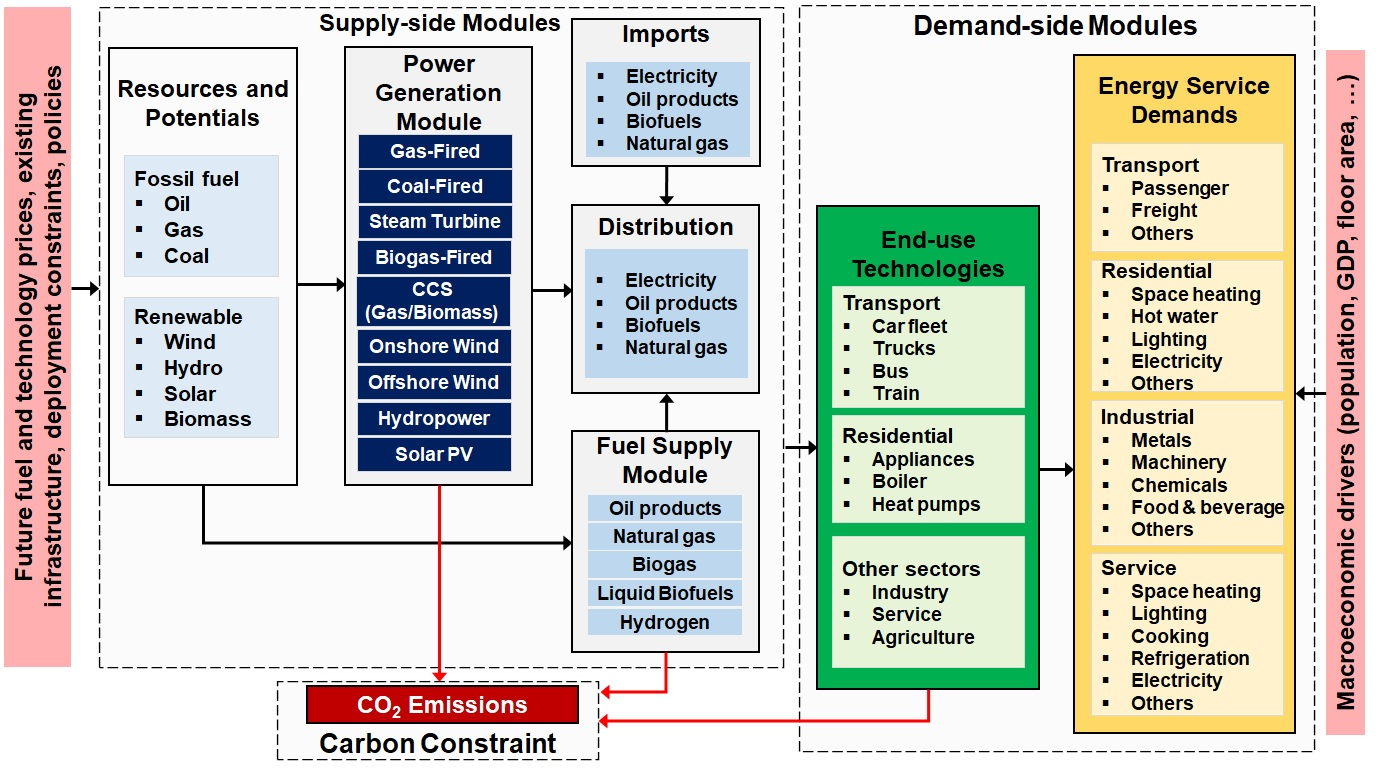
\includegraphics[scale=0.62]{TIM_RES.jpg} 
 \caption{Simplified representation of reference energy system in TIM}
 \label{fig:TIM-RES}
\end{figure}

The model's base year is 2018 and all energy flows, emissions and energy technology stocks are calibrated to SEAI's 2018 energy balance \citep{SEAI2019}.

The discount rate, the degree to which future values are discounted to the present, is a key parameter variable in the TIMES objective function. A social discount rate reflects how society views present costs and benefits against future ones and is lower than a financial discount rate, which is how firms make investment decisions. In appraising potential projects or investments, the Government applies a social discount rate. Broadly speaking, in an ESOM scenario with a carbon budget constraint, a higher discount rate would promote later decarbonisation and less capital-intensive technology choices. In this model, a discount rate of 4\% is applied, which is based on a Social Rate of Time Preference methodology as set forth in the Public Spending Code \citep{OCallaghan2018}. This rate is consistent with \citet{Garcia-Gusano2016} who recommend using a maximum value of 4-5\% for the social discount rate in ESOMs. 

Technology-specific discount rates (also known as hurdle rates) are typically used in ESOMs to capture investment decision-making from the individual user or industry perspective, to capture market imperfections, limited finance and behavioural heuristics which limit the uptake of novel or capital-intensive investments, even when they are cost-optimal. These parameters are not used in the core version of TIM given its use for modelling long-term energy system pathways from a societal perspective. However, future variants of the model can be developed to simulate real-world impacts of policies and behaviour which can include hurdle rates. 

\subsection{Time \& Geography}
\label{ss:time_geo}
TIM has been developed with a deep knowledge of the geography of the Irish energy system. A parametric spatio-temporal approach has been take in the RES base year specification and scenario file data structures to allow flexible regional definitions and temporal resolution within TIM. TIM can run in multiple modes with multiple configurations of regional and temporal resolution ranging from a single region national model at one annual time slice, all the way to 26 counties at hourly resolution where supply-demand data is available at that spatio-temporal granularity (Electricity, Gas \& Transport). Furthermore within the power sector each existing individual power plant turbine is modelled individually with unit commitment. High techno-temporal granularity is needed to appropriately model energy futures with high variable renewable energy systems integration, especially in scenarios with high levels of electrification of end use demands. High spatial granularity is required to give greater policy clarity on optimal investment needs based on regions and counties specific characteristics to enable counteracting socio-economic challenges such as energy poverty and infrastructure development within an optimisation framework. We have decided to focus on this data-driven spatio-temporal model setup to future-proof TIM and enable future Irish energy policy research needs as data-availability improves during TIM's lifespan. This trend has already begun with Gas Network data becoming available at hourly resolution at high spatial granularity.

\subsection{Demands: Drivers \& projections}
\label{ss:model_proj}
Energy service demands in end-use sectors are driven by growth in the population and in the economy. The model is set up to allow for alternative scenarios for these drivers to feed into energy service demand projections in the end-use sectors. This section describes baseline driver projections; detailed descriptions of energy service demand projections are in the respective sectoral sections. 
\subsubsection{Population}
Historical population estimates and future projections are obtained from the Central Statistics Office (CSO), Ireland \citep{CentralStatisticsOffice2020}. We use the M2F1 scenario since it represents medium growth in population and is in line with population projections used in other national sources \citep{Yakut2020}.

% Table generated by Excel2LaTeX from sheet 'Population'
\begin{table}[htbp]
 \centering
 \footnotesize
 \caption{Population}
 \begin{tabular}{cc}
 \hline
 Year & Population (millions) \\
 \hline
 2018 & 4.85 \\
 2020 & 4.98 \\
 2030 & 5.40 \\
 2040 & 5.82 \\
 2050 & 6.19 \\
 \hline
 \end{tabular}%
 \label{tab:pop}%
\end{table}%


\subsubsection{Economic growth}
\begin{itemize}
 \item Historical Gross Value Added (GVA) for the required NACE categories in the Services and Industry sectors is obtained from EUROSTAT database. Projections for GVA are outputs of the Ireland Environment, Energy and Economy (I3E) model \citep{Yakut2020}.
 \item Gross Domestic Product (GDP) - Historical and future projections for GDP is obtained from Organisation for Economic Co-operation and Development (OECD) \citep{OECD2018}. 
 \item Income - Historical values of total incomes are taken from CSO's database \citep{CSOincome}. Assumption about income growth in the future are that from the National Transport Model \citep{AECOMIrelandLimited2019}. 
 %\item Employment - The number of people employed in each of the NACE categories is obtained from EUROTSTAT database. Future projections are based on average levels of employment in the last decade with respect to the total population. 
 \item Modified Gross National Income (GNI*)- Derived from CSO's labour force scenario combined with a forecast for output per person \citep{cso_lf}. 
\end{itemize}

\subsubsection{Energy service demands}
Table \ref{tab:ESD_list} lists the energy service demands in TIM along with their corresponding drivers and values for 2018 and 2050. Specifics of the methodologies for projecting each energy service demand are detailed in later sections, for transport (\ref{ss:transport}), residential (\ref{ss:residential}), industry (\ref{ss:industry}) and services (\ref{ss:services}). 

% Table generated by Excel2LaTeX from sheet 'Sheet1'
\begin{table}[htbp]
\footnotesize
 \centering
 \caption{Energy service demands in TIM}
 \scalebox{0.9}{
 \begin{tabular}{p{18em}lccc}
 \hline
    \multirow{2}[0]{*}{Energy Service Demand} & \multirow{2}[0]{*}{Driver} & \multicolumn{2}{c}{Value} & \multirow{2}[0]{*}{Unit} \\
          &       & \multicolumn{1}{c}{2018} & \multicolumn{1}{c}{2050} &  \\ \hline
    Non-Energy Mining  & GVA per capita, Population & 2.07  & 0.13  & PJ \\
    Food and beverages  & GVA per capita, Population & 22.25 & 34.00 & PJ \\
    Textiles and textile products  & GVA per capita, Population & 1.20  & 4.97  & PJ \\
    Wood and wood products  & GVA per capita, Population & 6.69  & 7.65  & PJ \\
    Pulp, paper, publishing and printing  & GVA per capita, Population & 0.67  & 2.31  & PJ \\
    Chemicals and man-made fibres  & GVA per capita, Population & 10.60 & 13.11 & PJ \\
    Rubber and plastic products  & GVA per capita, Population & 1.14  & 0.89  & PJ \\
    Other non-metallic mineral products  & Modified investment, GNI* & 17.77 & 24.82 & PJ \\
    Basic metals and fabricated metal products  & GVA per capita, Population & 19.54 & 21.73 & PJ \\
    Machinery and equipment n.e.c.  & GVA per capita, Population & 1.29  & 1.69  & PJ \\
    Electrical and optical equipment demand & GVA per capita, Population & 4.27  & 16.37 & PJ \\
    Transport equipment manufacture  & GVA per capita, Population & 0.17  & 0.04  & PJ \\
    Other manufacturing  & GVA per capita, Population & 4.25  & 6.12  & PJ \\
    Construction & GVA per capita, Population & 4.02  & 5.90  & PJ \\
    Transport Demand: Short-range passenger travels & Income, population & 14.56 & 21.07 & BPKMS \\
    Transport Demand: Medium-range passenger travels & Income, population & 31.28 & 45.29 & BPKMS \\
    Transport Demand: Long-range passenger travels & Income, population & 27.13 & 38.97 & BPKMS \\
    Transport Demand: Goods vehicle for freight & Growth rate from \citep{AECOMIrelandLimited2019} & 11.54 & 25.14 & BTKMS \\
    Transport Demand: Turism fuel  &       & 7.72  & 0.00  & PJ \\
    Transport Demand: Navigation fuel  & GDP   & 3.51  & 10.04 & PJ \\
    Transport Demand: Unspecified fuel &       & 21.78 & 0.00  & PJ \\
    Transport Demand: Aviation domestic &       & 0.23  & 0.23  & PJ \\
    Transport Demand: Aviation international & International Aviation Passengers & 45.94 & 62.63 & PJ \\
    Residential Apartment Demand & Population & 206.80 & 628.93 & 000' \\
    Residential Attached Demand & Population & 766.35 & 1056.50 & 000' \\
    Residential Detached Demand & Population & 724.43 & 889.76 & 000' \\
    Services - Commercial Services & GNI*  & 28.90 & 47.39 & Mm\textsuperscript{2} \\
    Services - Public Services & GNI*  & 58.15 & 95.35 & Mm\textsuperscript{2} \\
    SRV-Commercial Services: Data centers & From EirGrid & 5.63  & 40.30 & PJ \\
    SRV-Public Services: Public lighting & From \citep{GovernmentofIreland2018} & 0.48  & 0.58  & Mlamps \\ \hline
    \end{tabular}%
    }
  \label{tab:ESD_list}%
\end{table}%


\subsection{Development approach}
\label{ss:model_dev}

%Git and related toolbox. 
%- web app
%- open data, open source
%- version control (cite papers if possible)

TIM has been developed with the goal of achieving ``best practice" standards in software development and open modelling convention. A git-centred model development process has been an integral part of the model development approach to enable version control and model management. Along with improvements in management, quality assurance and transparency this brings, it also allows developers and researchers from different projects to branch research versions of the model, to explore innovations and new developments, while keeping a secure and stable main version of the model for policy application. At the same time, individual projects and researchers can input their improvements and developments to the core model, to enable continuous improvements. 

TIM is openly available, which is a prerequisite for transparency, repeatable research, model maintenance and enhancement and verification of results \citep{Pfenninger2018}. 

Web-based dashboards\footnote{https://tim-review1.netlify.app/results/} have been extensively used in the model development process, both for internal model diagnostics and for external engagement and review. 

TIM has been co-developed with the LEAP-Ireland model \citep{MacUidhir2020}, which is a bottom-up simulation model of the Irish energy system which simulates the impact of different policy measures and targets on overall GHG emissions in Ireland, with a particularly granular representation of transport and residential heat demand. Underlying data for the relevant sectors are shared between TIM and LEAP using a Data Repository and shared coding convention dictionary to improve the consistency between the models, give more robust analytical insights for policy and to share and exchange expertise between the modelling teams. This also facilitates multi-model approaches to energy systems modelling, which can make use of harmonised hybrid frameworks coupling simulation and optimisation simultaneously \citep{rogan2014leaps}.

TIM has also been developed to enable soft-linking with the Ireland Environment, Energy and Economy (I3E) macroeconomic model developed at the Economic and Social Research Institute (ESRI) \citep{Yakut2020}. I3E is a single-country, multi-sector (NACE) inter-temporal computable general equilibrium (CGE) model focusing on environmental and energy accounts in Ireland. While COre Structural MOdel for Ireland (COSMO) focuses on the influence of monetary and fiscal policy on economic activity in Ireland, I3E supplements the macroeconomic outlook from COSMO with environmental and energy disaggregation. I3E retrieves economic growth rates and population estimates from COSMO. TIM derives macroeconomic drivers coupled to the output variables of I3E, enabling scenario variants based on alternative monetary, fiscal and macroeconomic futures. The coding conventions, datahub, and linking to original raw data approach, enables rapid energy system outlook updates aligned with the update cycle of the macroeconomic outlooks from the ESRI, Central Bank and OECD.

%TIM has also been developed to enable wide stakeholder review, feedback and iterative policy insight. %Will write this for the paper - after the review process. 

\section{Sectors}
\label{s:sectors}

\subsection{Supply}
\label{ss:supply}
\subsubsection{Overview}
The supply sector (SUP) in TIM represents the primary and secondary energy commodities and the processes by which those same commodities are imported, exported, domestically produced through mining or capture of renewable energy potentials and transformed or refined for end-use consumption within the energy system both in the base year (2018) and into the future. The supply sector declares the future available routes for commodity trade for import and export of energy commodities in terms of quantity of energy, and in terms of import capacity through ports, pipelines and inter-connectors at any given time in the model horizon. 

\subsubsection{Energy Balance and Commodity Declarations}
Building the supply sector begins with declaring the energy commodities as per the SEAI energy balance as reported to the international energy agency \citep{SEAI2019}. Attention is taken to ensure best practice coding conventions are followed for each commodity - coal, oil, gas, first- and second-generation bioenergy (biogas, bioliquids and solid biomass), liquid and gaseous hydrogen, wind, solar, geothermal, wave, tidal, municipal wastes, agriculture wastes, industrial food waste. Active transport time for walking and cycling is also declared. Setting out predefined and intuitive commodity naming convention and a dictionary that is shared across TIM and LEAP-Ireland has multiple benefits for multi-model coupling, diagnostics and results reporting that is discussed. All base year commodities are declared in the Supply sector to maintain clear, tidy and transparent data structures within TIM.

\subsubsection{Emissions Tracking}
The environmental emissions from each primary energy commodity is tracked on the basis of energy and processed based emissions via combustion and activity based emissions intensity factors, calibrated on an sector-by-sector basis. Within the Supply sector, methane, nitrogen dioxide, sulfur dioxide, carbon dioxide, nitrogen oxide, and particulate matter (PM2.5, PM10) are tracked in the sector's emissions accounting balance.

\subsubsection{Import/Export}
Primary and secondary energy commodities, both fossil energy and bioenergy, are imported from international markets at international prices. There are no constraints on the import quantity of oil and coal as it is assumed that international markets can supply domestic demand and that there is sufficient on island storage aligned with IEA-OECD energy security protocols. Imported gas via pipeline and LPG are modelled on a seasonal basis and are constrained to reflect seasonal peak import capacity constraints in pipelines. Bidirectional electricity inter-connectors to the UK are also declared in the upstream supply sector.

\subsubsection{Fuel prices}
Fuel prices for each imported energy commodity are sourced from the International Energy Agency's World Energy Outlook (WEO) from 2019 and 2020 \citep{InternationalEnergyAgency2020}. Secondary commodity import prices are index linked to the primary commodity by a price ratio on the basis of the current ratio between primary and secondary prices. For example, imported gasoline is assumed to be 1.65 times the price of crude oil per unit energy.


\subsubsection{Domestic Energy Resources}
Domestic fossil fuel reserves for production of natural gas from both the Corrib and Kinsale gas fields, and the production of peat, are calibrated with two-step supply curves. These supply curves are constrained in terms of cumulative energy reserves, annual production costs, and annual production output in energy terms to account for typical production profiles from each field.

Renewable energy potentials (hydro, wind, solar, waste, ocean, geothermal, and ambient heat) are declared in the upstream sector but are calibrated and constrained in their relevant sectors, such as power generation and transport.

\subsubsection{Bioenergy potentials}
Bioenergy potentials are calibrated to the SEAI's ``Bioenergy Supply in Ireland: 2015-2035" report \citep{SEAI2015} both in terms of sustainable import volume availability and domestic production potentials. Domestic bioenergy potentials such as sawmill residues, post-consumer recycled wood, municipal waste, tallow, recovered vegetable oil, straw, animal waste and industrial food wastes are modelled with three-step supply curves in terms of price and quantities available. Crop-based bioenergy feedstocks are modelled within the agriculture sector. Domestic bioenergy supply potentials and costs are sensitive to scenarios narrative and as such are modelled within scenario files to account for uncertainty.

Available agriculture sector commodities both bioenergy, land availability and herd types are declared in the supply sector.

\subsubsection{Refineries}
The Whitegate refinery is calibrated to import crude oil at international prices and converts crude oil to the refineries typical fuel slate based on upper bounds of fuel shares such that the output has flexible upper shares of 22.9\% gasoline, 8.1\% kerosene, 40.9\% diesel with the remaining 34.4\% heavy fuel oil to be exported with an overall conversion efficiency of 99.2\%. The refinery is constrained to stay at current capacity, has a lifespan of 50 years, and the production costs are differentiated by production (flow) costs for each output fuel.

\subsubsection{Electricity Inter-connectors}
Existing electricity inter-connectors are calibrated such that there is a price differential between annual average price for import or export of electricity to the UK of \euro{4}/GJ. The 2018 export quantity of electricity to the UK is calibrated as per historical data, but export activity of electricity is currently a weakness in the model given that TIM does not model the UK electricity market, other than a price signal, and so future imports and exports of electricity is constrained off by default. This constrained can be relaxed but is used to explore domestic needs for system flexibility, security, system services, and storage in terms of hydrogen and battery electricity storage.

\subsubsection{Biorefineries}
Future bio-refinery technologies are defined in the supply sector future technology (SubRES) database. Ethanol production from wheat, woody biomass and grass is defined. Bio-diesel options from OSR, woody biomass, industrial food waste, RVO and tallow are defined. Wood pellets from biomass is defined. Biogas production from Grass, woody biomass, Municipal waste, industrial food waste and animal wastes are defined. All bio-refining technologies are defined in terms of potential start year, efficiency, investment costs, their availability factor and the operation and maintenance costs.

\subsubsection{Hydrogen}
Hydrogen production is modelled in the future, disaggregating centralised and decentralised electrolysis options. Delivery options are disaggregated and costed at high pressure for both transmission and distribution pipelines as well as a road tanker option for distribution. Hydrogen storage is also modelled within TIM at the DAYNITE timeslice level allowing hourly production and consumption of hydrogen to be modelled. This is particularly useful for modelling electricity grid balancing with unit commitment, dispatch and capacity expansion while capture variable renewable energy system dynamics. We will discuss this further in the power sector description. 

\subsection{Electricity}
\label{ss:power}

\subsubsection{Overview}
Ireland has a high share of variable renewable electricity for a relatively isolated grid, with 32.5\% of electricity generation in 2019 coming from onshore wind energy. Achieving the 2020 RES-E target has encouraged strong growth in onshore wind, while increasing the non-synchronous penetration of renewables to 70\% by 2030 including offshore wind development is a key policy objective over the next decade as Ireland moves towards a net zero carbon electricity system. 

Due to computational burden, existing long-term ESOMs mainly apply stylised temporal resolution and split each model year into 10 to 20 time-slices. This level of temporal resolution is insufficient in capturing implications from variable renewable energy sources with high intermittency, causing inaccuracy in modelling results, including generation capacity, energy storage, and additional cost related to requirements in flexibility options. Previous analysis has applied new methodologies to address the weakness of energy systems modelling in treating short-term constraints \citep{Collins2017}. For example, a soft-linking methodology has been applied to link Irish-TIMES model with a unit commitment and economic dispatch models such as PLEXOS \citep{Deane2012}. With high technical and temporal details, the PLEXOS model better simulates the operation of the power system and provides additional insights into the power system. However, soft-linking methods do not assure convergence and optimality of such incoherent modelling framework. Some analysis has improved temporal resolution and demonstrated that increasing the number of time slices has impacts on modelling results \citep{Pina2011,Kannan2013,Gaur2019}. However, it is pointed out that only increasing time slices may not be enough and there are other impacting factors \citep{Poncelet2016}. The TIM power sector provides an integrated modelling framework with high temporal, spatial and technical resolution that better model the operation of the power system hard coupled into the overall energy system to capture implications from variable renewable energy sources under deep decarbonisation pathways. 

The TIM power sector has been developed with state-of-the-art TIMES modelling methods including several novelties, such as flexible regional definitions, flexible time-slice definition (up to an hourly resolution with 8760 time-slices), ability to model dispatch, unit commitment of individual generation units, capacity expansion, and spatially explicit grid connection supply curves cost of future onshore wind potential. Modelling with TIM in hourly unit commitment mode further enables intra-day and inter-day energy storage options to be modelled appropriately leveraging pumped hydro, hydrogen production and consumption and battery electric technology options in the future technology (SubRES) database. This enables TIM to be able to appropriately model the challenges of integrating high levels of variable renewable electricity onto a relatively isolated grid, while balancing supply, curtailment, and energy storage with demand growth in historical sectors as well as new demands for power such as data centres.

\subsubsection{Existing Dispatchable Grid}
It is well documented in the literature that ESOMs that do not include reasonably high temporal resolution and unit commitment details typically over estimate the potential for VRES in future zero carbon energy systems and under-estimate the requirement for energy storage and system flexibility on the grid.

The existing 61 generation unit fleet is calibrated to the base year of 2018 from the Commission for Energy Regulation (CRU) I-SEM validated PLEXOS model \citep{Geffert2018}. Each existing generation unit can be explicitly modelled with unit commitment. This model configuration includes the generation unit capacity, the fuel type of each generation unit, the start up costs (from cold, warm and hot), the efficiency curve of the generation unit to include startup and shutdown phases, startup and shutdown times (cold, warm and hot), the ramp rates, minimum load, efficiency at minimum load, minimum up-time and minimum down-time, the unit lifespan, the unit annual availability, and the start year of the unit \citep{Geffert2018}. The near-term generation unit pipeline is calibrated to the 2020 Eirgrid Generation Capacity Statement (GCS) to account for early closures of units before their economic lifespan, which largely takes into account coal and peat based plants during the next decade \citep{EirGridadSONI2019}. We have not forced on new capacity of future planned power plants from the GCS in TIM, which includes recent battery storage installations. These recent and planned units can be forced on via a scenario file. 

The existing 302 Onshore and 1 Offshore Wind farms within the Irish Wind Energy Association database currently operate as a single aggregated generation pool governed by historical hourly availability factors for wind generation from 2018.

\begin{figure}[!htbp]
 \centering
 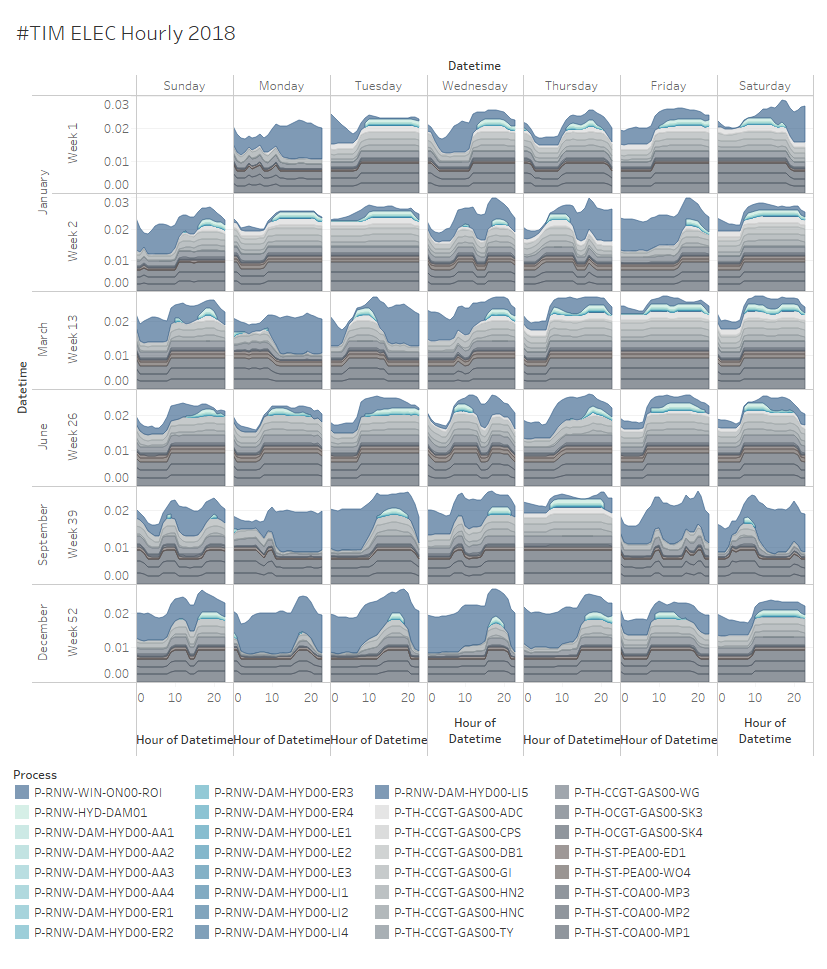
\includegraphics[scale=0.6]{TIM_Elec_Hourly (2).png} 
 \caption{TIM hourly unit commitment modelling capabilities example for 2018}
 \label{fig:TIM_HourlyELC}
\end{figure}

\subsubsection{Future Electricity system}
New generation capacity investment costs, fixed and variable operation and maintenance costs and technical efficiencies are derived from the European Commission's Joint Research Centre (JRC) Energy Technology Reference Indicator projections for 2010-2050 \citep{Carlsson2014}. The future unit commitment dispatch operational constraints and cycling costs are generalised for each technology type based on fuel and vintage \citep{Kumar2012}. 

Renewable energy potentials are based on a number of sources: Total energy resource availability of solar and wind are from \citep{Pfenninger2016} and \citep{Staffell2016} respectively with availability factors from \citep{Ruiz2019}. Ocean energy, tidal energy potential is from \citep{ORourke2010} and wave energy power matrix is derived from \citep{Nambiar2016}. Hourly availability factors for ocean energy technologies are derived from the marine institute and OPW's data buoy services.

Future onshore wind energy potential has been assessed at high spatial resolution using GIS techniques. Wind farm expansion is constrained by both technology costs and a supply curve for grid connections based on a GIS analysis of existing houses, special areas of heritage and conservation, existing grid lines by voltage specification, wind energy potential, existing substation locations, and the costs per kilometre of standard ESB grid line specifications to connect wind resource potential to the existing grid. The wind energy potential is defined as a cost curve aggregated from the original 1938 suitable land parcels from the GIS analysis. (Fig. \ref{fig:wind-onshore-potential}). Due to the fact that increasing both technical details and temporal resolution causes exponential increase in model size, the spatial resolution is simplified and is represented in a 4 step cost curve (Fig. \ref{fig:wind-conn}). this can be dissaggregated on a spatial resolution down to each individual parcel of land, or on a county by county basis. Future hourly wind energy generation can generate at the same hourly capacity factor that occurred in 2018, however with capacity expansion.

Losses from electricity transmission and distribution are assumed to be 7\%, with no grid expansion costs currently represented in the model. The maximum share of variable renewable energy including wind, solar and wave energy is constrained at 75\% by 2030 and 100\% is allowed by 2050. 

\begin{table}[h]
 \centering
 \footnotesize
 \caption{Onshore wind connection cost }
 \begin{tabular}{cc}
 \hline 
 Capacity(GW) & Connection Cost (Euro/kw)\\ 
 \hline
 0-8.1 & €25 \\
 
 8.1-16.8 & €39 \\
 
 16.8-22.6 & €69 \\
 
 22.6-26.6 & €153 \\
 
 26.6-30.6 & €358 \\
 
 \hline
 \end{tabular}
 
 \label{onshore-wind-connection-cost}
\end{table}

\begin{figure}[!htbp]
 \centering
 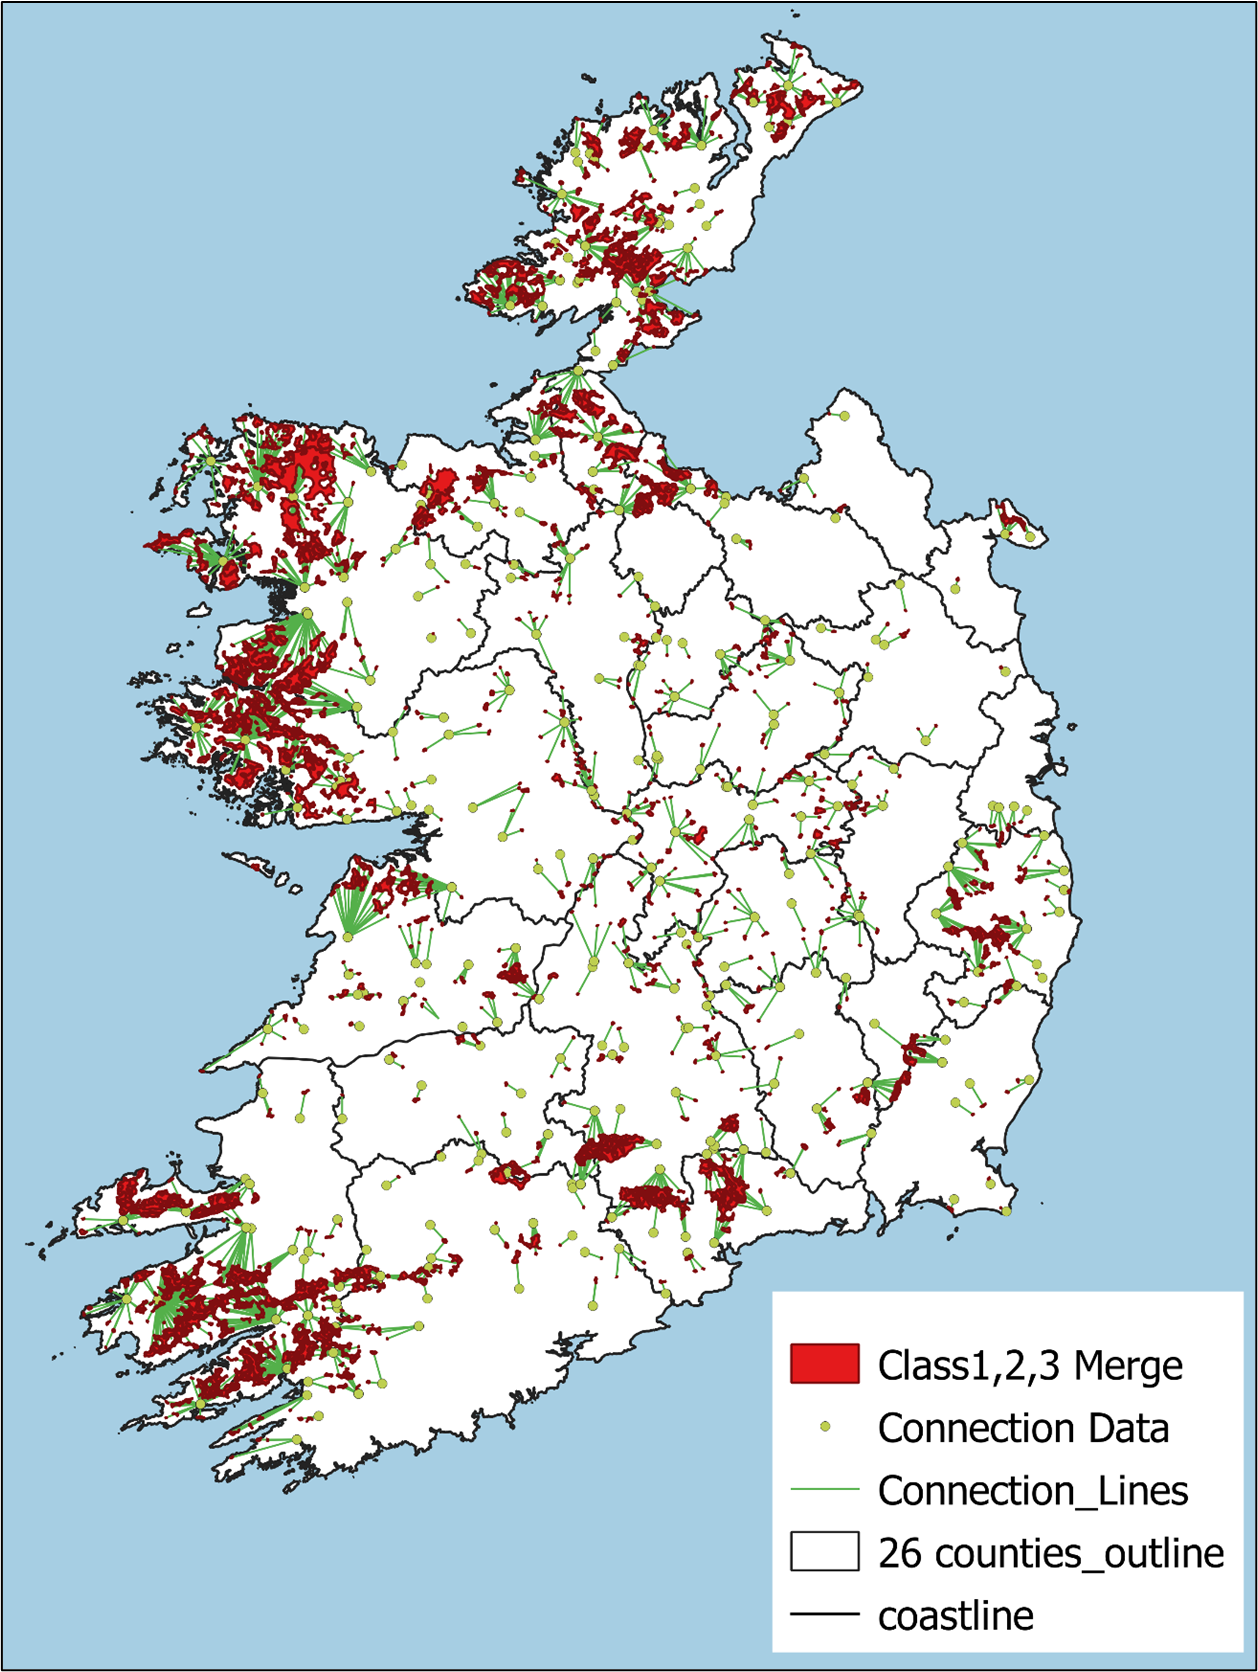
\includegraphics[scale=0.6]{WindPotentialMap.png} 
 \caption{Wind energy potential locations}
 \label{fig:wind-onshore-potential}
\end{figure}

%\begin{figure}[H]
% \centering
% 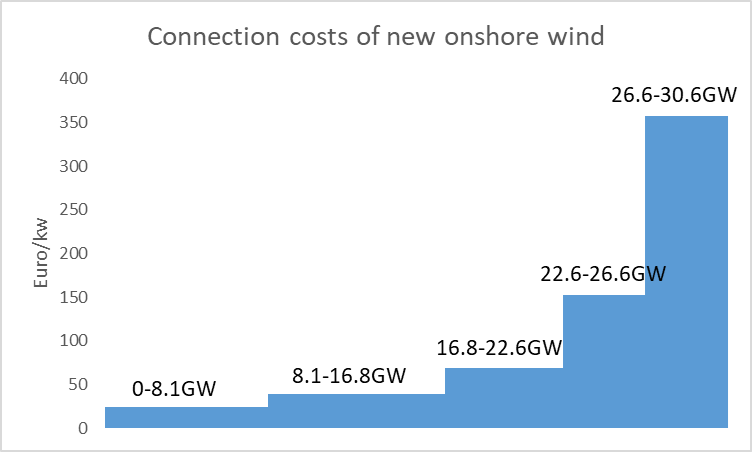
\includegraphics[scale=1]{stepwise-connectioncost.png} 
% \caption{Connection cost of new onshore wind}
% \label{fig:wind-conn}
%\end{figure}
%Xiufeng can you provide xls please? 

\subsubsection{Carbon Capture and Storage, Carbon Dioxide Removal, and Negative Emissions technologies}
It is well documented in the literature that residual emissions are likely to remain in the future (net) zero carbon energy system from ``hard-to-decarbonise" sectors \citep{Rogelj2018}. Carbon Capture and Storage (CCS), Carbon Dioxide Removal technologies (CDR), and Negative Emission Technologies (NETS) are currently seen within the literature as critical future technologies to capture the last marginal residual emissions to bring the energy system to net-zero CO2 or even net-negative CO2 by mid-century. With this in mind, TIM has carbon capture and storage (CCS) technology options available from 2030, including retrofit options on existing coal, peat and gas power plants. Bioenergy carbon capture and storage (BECCS) is defined available in TIM from 2030 and provides net negative CO2 capture and allows negative emissions electricity generation. Direct air carbon capture and storage (DACCS) is also defined as a backstop technology but will be appropriately calibrated to best practice approaches in the future technology database (SubRES) \citep{Realmonte2019}. CCS is also available in some ``hard-to-abate" industrial sectors such as cement production.

\subsubsection{User constraints}
User constraints applied to the Power sector in TIM largely pertain to the calibration of the near-term shutdown of coal and peat power plants before their economic life-time ends as a result of policy decisions. 

\subsection{Transport}
\label{ss:transport}

\subsubsection{Overview}
The transport sector comprehensively describes the end-use transport technologies, and freight and mobility demands on a regional basis. This sector is divided into 26 counties across Ireland. To represent region-specific transport characteristics, some main parameters (vehicle fleet, transport infrastructure, fuel consumption, mileage, occupancy rate, load factor) are differentiated on a county level. Transport demand is split to three main categories: passenger, freight, and others. The passenger and freight demands are expressed as activity demands, and others are defined as a final energy demand (PJ). These final energy demands further split into aviation (international and domestic), navigation, fuel tourism and unspecified, aligned with the SEAI Energy Balance \citep{SEAI2019}. ``Fuel tourism" refers to cross-border consumers and a portion of demand is used by unspecified modes. 

The passenger transport demands are expressed in billion-passenger kilometres (Bpkm). As shown in Table \ref{passenger transport demand}, the total passenger demand is divided into three classes of distance range including short-range (less than 5km), medium-range (5-30 km), and long-range (more than 30km) \citep{NTA2018}. Moreover, four transport modes satisfy travel demands including 1. public services (bus, train, taxi), 2. private cars, 3. two-wheelers, and 4. active modes (walk and bike). For simplification, non-motorised transport is only used for short-range trips, 2-wheeler are used for short- and medium-range travels, urban bus and school bus are used for short- and medium range travels, Intercity bus and heavy train are used for long-range trips, and light rail can only use for the short- and medium-range trips in Dublin county. As shown in Fig. \ref{fig:TRA-TIM}, demand for each mode can be met with a different set of technologies based on cost-optimisation and user constraints. The base year is calibrated based on the actual number of vehicles and the corresponding vehicle activities. Table \ref{vehicle stock} shows the characteristics on a national basis. 

\begin{table}[h!]
 \centering
 \footnotesize
 \caption{Total passenger demand and share of transport modes for each class of distance range \citep{CentralStatisticsOffice2020a, CentralStatisticsOffice2020b, CentralStatisticsOffice2020c, CentralStatisticsOffice2020d, CentralStatisticsOffice2020e, CentralStatisticsOffice2017}}
 \begin{tabular}{lllll}
 \hline 
 Modes & Vehicles & \makecell{Short-range \\ (below 5km)} & \makecell{Medium-range \\ (5-30km)} & \makecell{Long-range \\ (over 30km)} \\ 
 \hline
 Public & Bus & 8.3\% &	13.5\% &	16.1\% \\
 & Light train &	0.8\% &	0.7\% &	NA \\
 & Heavy train &	NA & NA &	8.4\% \\
 & Taxi &	1.7\% &	2.2\% &	1.3\% \\
 \hline
 Private & Cars	& 51.5\% &	83.3\%	& 74.2\% \\
 \hline
 2-wheeler & Motorcycle & 0.1\% &	0.3\%	& NA \\
 \hline
 Active & Bike &	5.4\% & 	NA & 	NA \\
 
 & Walk &	32.2\% &	NA &	NA \\
 \hline
 \multicolumn{2}{c}{Total passenger demand in 2018 (Bpkm)} &	14.6 &	31.3 &	27.1 \\ [1ex]
 \hline
 \end{tabular}
 
 \label{passenger transport demand}
\end{table}


The inland freight demands are expressed in billion-tonne kilometres (Btkm). It comprises two main modes: goods trucks and train. The definition of light and heavy goods vehicles varies in different studies. In this model, they are disaggregated by three unladen weight bands: light-duty trucks (below 5 tonnes), medium-duty trucks (5-10 tonnes) and heavy-duty trucks (over 10 tonnes) \citep{CentralStatisticsOffice2020d,CentralStatisticsOffice2020e,CentralStatisticsOffice2020f}. Table \ref{ton-km} shows the freight demand in the base year. 

\begin{table}[h]
 \centering
 \footnotesize
 \caption{Freight demand in 2018 \citep{ CentralStatisticsOffice2020d, CentralStatisticsOffice2020e, CentralStatisticsOffice2020f}}
 \begin{tabular}{llll}
 \hline 
 Classification & Unladen weight & Demand (mtkm) & Share\\ 
 \hline
 Light-duty trucks & 0-5 tonne & 292 & 2.5\% \\
 
 Medium-duty trucks & 5-10 tonne & 1140 & 9.8\% \\
 
 Heavy-duty trucks & over 10 tonne &	10106 & 86.9\% \\
 
 Train & - &	89 & 0.8\% \\
 
 \multicolumn{2}{l}{Total Freight demand} & 11627 & 100\% \\ \hline
 \end{tabular}
 
 \label{ton-km}
\end{table}

\begin{figure}[h!]
 \centering
 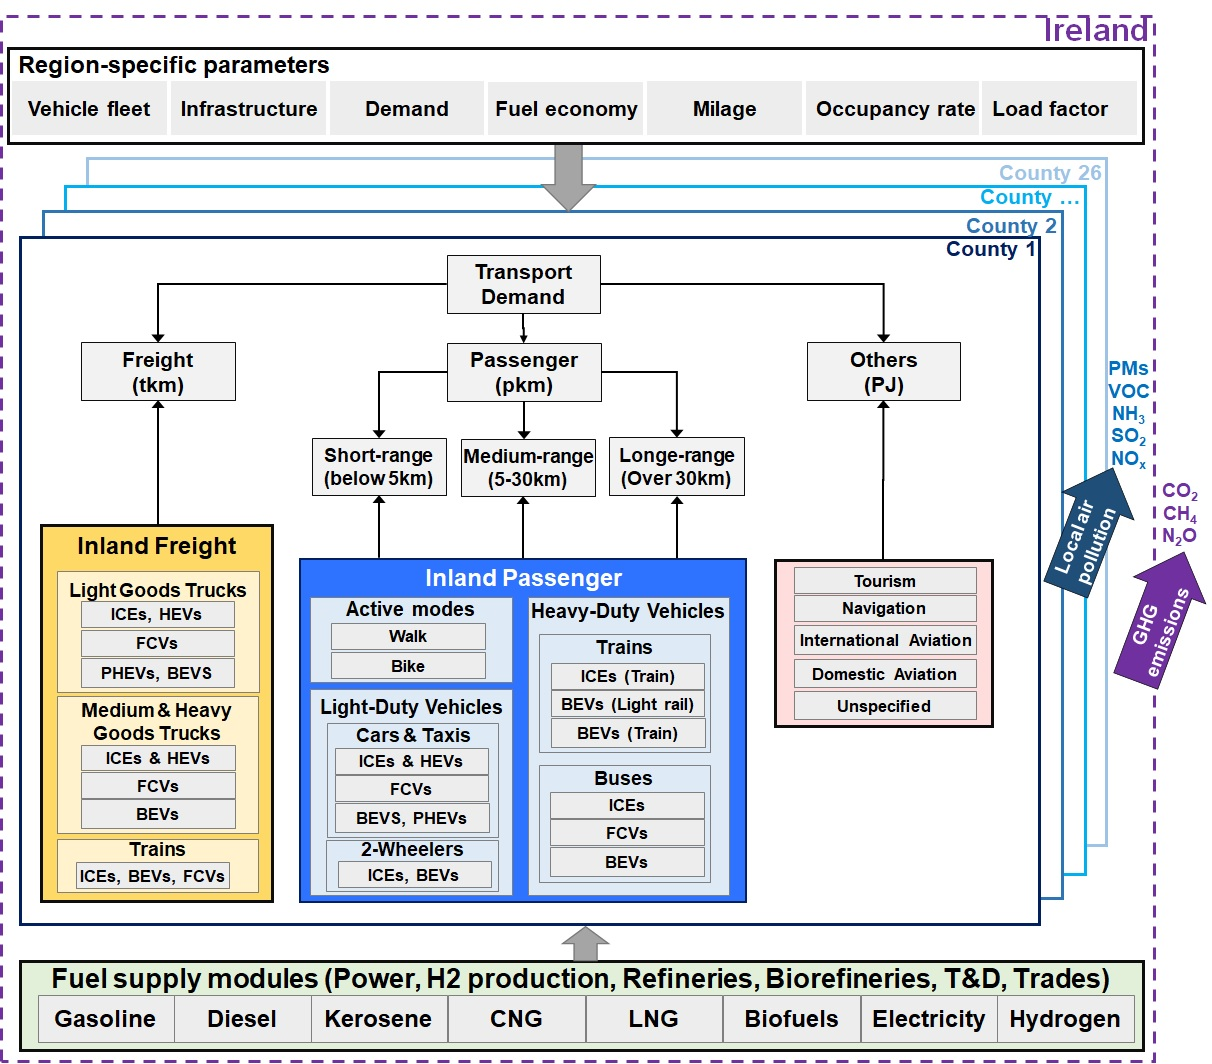
\includegraphics[scale=0.60]{Transport in TIM.jpg} 
 \caption{Transport structure in TIM}
 \label{fig:TRA-TIM}
\end{figure}

\begin{table}[h]
 \centering
 \footnotesize
 \caption{Existing vehicles and the corresponding characteristics in the base year \citep{CentralStatisticsOffice2020g, CentralStatisticsOffice2020h, CentralStatisticsOffice2020i, IrishRail2018, TransportInfrastructureIreland2016}}
 \scalebox{0.9}{
 \begin{tabular}{llllll}
 \hline 
 Vehicles & Powertrain & \makecell{Stock\\ (000-Units)} & \makecell{Utilisation \\ factor \\(1000km/yr)} & \makecell{Occupancy \\rate\\ (Pass./Vehicle)} & \makecell{ Fuel\\ consumption\\ (MJ/v.km) }\\ 
 \hline
 Motorcycle & Gasoline ICE & 39.85 &	2.73 &	1.10 &	1.70\\
 \hline
 Cars &	Gasoline ICE &	946.86 &	12.82 &	1.49 &	2.47\\
	 & Diesel ICE & 1129.40 &	20.62 &	1.49 &	2.30\\
	 & Dual-fuel ICE &	0.07 &	13.44 &	1.49 &	2.89\\
	 & ICE-E85 &	8.53 &	13.44 &	1.49 &	2.41\\
	 & Gasoline HEV &	29.80	& 12.82	& 1.49 & 2.05\\
	 & Diesel HEV &	0.77 &	20.62 &	1.49 &	2.03\\
	 & Gasoline PHEV &	2.76 &	12.82 &	1.49 &	1.56\\
	 & Diesel PHEV &	0.03 & 20.62 &	1.49 &	1.58\\
	 & BEV &	4.53 &	13.44 &	1.49 &	0.85\\
	 \hline
 Taxi &	Gasoline ICE &	2.50 &	35.61 &	1.49 &	2.63\\
	 & Diesel ICE &	17.46 &	39.93 &	1.49 &	2.39\\
	 & Gasoline HEV & 	1.35 &	41.21 &	1.49 &	2.03\\
	 \hline
 Bus &	Diesel-ICE & 10.70 &	36.10 &	27.25 &	10.16\\
 \hline
 Train &	Light train (Electric) & 0.07 &	55.69 &	78.0 & 24.81\\
	 & Heavy train (Electric) &	0.05 &	158.48 & 78.0 &	24.81\\
	 & Heavy train (Diesel) &	0.014 &	73.88 &	120.0 &	76.92\\ [1ex]
 \hline 
 \end{tabular}
 }
 
 \label{vehicle stock}
\end{table}

\subsubsection{Future transport demand projections}
\subparagraph{Passenger kilometres: Private Cars}
Future passenger car transport demand is projected based on future population growth and a growing rate of car ownership, which is in turn determined by income growth. Car ownership usually follows an S-shaped function which has three periods: slow growth during low income levels, rapid increase as income levels rise quickly and finally a saturation period. Gompertz statistical model has been found to best fit the historical relationship car ownership and income levels, although other functions have also been used in previous studies \citep{Lian2018}. The basic Gompertz function is shown in Equation \ref{gompz_func}.
\begin{equation}
\label{gompz_func}
 y=\alpha*e^{-\beta*e^{-\gamma x}}
\end{equation}
here $y$ is the car per adult, $\alpha$ is saturation level of car ownership, $x$ is an economic indicator (income per adult in this case) and $\beta$,$\gamma$ are parameters that are estimated using historical data obtained from CSO. 

Projection of future car ownership levels is based on change in income levels. The saturation level of car ownership in this study is 875 per 1000 adults \citep{AECOMIrelandLimited2019}. Car ownership (car per adult) is projected to rise from 0.56 in 2018 to 0.69 in 2050, an increase of 23\%. Passenger kilometres are then derived using car ownership as a proxy and assuming an occupancy level of 1.492 and kilometres per car to remain constant at about 17300 per year. Total passenger kilometres from private cars is projected to increase by 42\% in 2050 from 2018 levels with a Compound Annual Growth Rate (CAGR) of 1.1\%. The growth rate of passenger kilometres from private cars was 1.35\% between 2008 and 2018. 

\subparagraph{Passenger kilometres: Other modes of transport}
Other modes of transport represent a much smaller share of mobility demand than that of private cars. Passenger kilometres of large public service vehicles (PSVs) are projected using population as a driver in a log function and assuming average occupancy of 27.5. Large PSV passenger kilometres are expected to increase by 24.2\% in 2050 as compared to that in 2018 with a CAGR of 0.7\%. Passenger kilometres of other modes such as luas, train, small PSVs, motorcycles and active modes such as walking, cycling are projected using population and year as the drivers. The passenger kilometres are expected to increase by 60\% with a CAGR of 1.5\%. 

\subparagraph{International Aviation fuel demand}
International aviation fuel demand is projected using number of passengers as the driver. The number of aviation passengers is forecast using damped Holt Winters function based on historical time-series data that is obtained from CSO \citep{Dantas2017,Grubb2001}. The number of passengers is expected to increase by 45.5\% in 2050 as compared to 2018. The historical fuel demand for aviation and number of aviation passengers are then used as an input for a linear regression model to project the future demand for aviation fuel. The fuel demand increases by 37\% in 2050 relative to 2018 with a CAGR of 1\%. 

\subparagraph{Other transport fuel demand}
Demand for freight is projected using growth rates available in \citep{AECOMIrelandLimited2019}. The growth in tonne kilometres of freight is expected to increase by 1.18 times in 2050 from 2018 level with a CAGR of 2.5\%. Navigation fuel demand is projected using GDP as the explanatory variable. Fuel demand for navigation is expected to increase 2.85 times in 2050 as compared to 2018 with a CAGR of 3.3\%. Fuel tourism is assumed to be constant at 11 PJ. 

\subsubsection{Future technology options}

Common vehicle technologies and future options that are likely to become available for future investment shape technology database for the transportation sector in TIM. They are categorised in five major groups \citep{Aryanpur2015}:
\begin{enumerate}
 \item Internal Combustion Engines (ICEs), consists of spark ignition engines fuelled by gasoline, bioethanol, CNG, BioCNG, hydrogen and dual-fuel engines (running either on gasoline or CNG/BioCNG, each one taking 50\% of the distance travelled), and compression ignition engines powered by diesel and biodiesel. 
\item Hybrid Electric Vehicles (HEVs) are equipped with an ICE, which provides the main power, and a small electric motor to support the ICE and to recuperate the braking energy. 
\item Plug-in Hybrid Electric Vehicles (PHEVs) have a similar powertrain to HEVs. But their batteries can be charged from the grid for driving tens of miles solely on electrical power. We assume the maximum distance that would be driven on electric mode is 50\% in the base year and it can increase to 80 percent over the study period. 
\item Battery Electric Vehicles (BEVs) solely rely on batteries, which provide the total motive power of the vehicle. The batteries are charged from electricity grid. 
\item Fuel Cell Vehicles (FCVs) are electrochemical devices that produce electricity through a reaction between hydrogen and oxygen. The electricity drives a vehicle’s electric motor. Conventional fuel tank is replaced with a pressurised hydrogen storage tank in FCVs. 
\end{enumerate}

Table \ref{vehicle-purchase} shows techno-economic characteristics of future passenger transport vehicles \citep{Mulholland2017,Helgeson2020}. Maintenance costs are assumed to remain constant. However, in some scenarios vehicle purchase price parity between BEVs and ICEs is expected in the period 2025-2030. 

All these technologies compete to meet the mobility demand over the planning horizon. The model structure allows competition among stock replacement and fuel substitution within a mode. Modal shift may be simulated within each travel distance band. 

Different fuels are supplied to the transport sector via four separated modules including supply, power, bio-refineries, and hydrogen modules. In other words, these connections integrate the transport sector with the entire energy system.

TIMES models usually use a simplified constant lifetime for different vehicles and thus, the vehicles are retired at the end of the lifetime. However, a detailed analysis of technologies’ retirement profile in Ireland shows that this simplified representation is far from reality. The actual profile shows a low decay in the beginning years and a long tail in the distribution over long-time. To improve the retirement profile both for existing and new vehicles, TIM is equipped with realistic representation of the survival profile of car technologies. The survival rates are from Irish CarSTOCK model \citep{daly2011modelling, Mulholland2018}. 

\subsubsection{User constraints}

A set of constraints limits fuel and modal shares in transport sector as follows: 
\begin{itemize}
 \item Maximum biodiesel share in passenger and freight transport demand is 4.1\% in the base year
 \item Maximum bioethanol share in passenger and freight transport demand is 3.2\% in the base year
 \item Modal share of passenger and freight transport as stated in Table \ref{passenger transport demand} and Table \ref{ton-km}, respectively. 
 \item Maximum growth rate in new vehicle sales for advanced powertrains (HEVs, PHEVs, BEVs and FCVs) is 30\% per year, which is enforced once the market share of a vehicle type reaches 10\%.
 \item The blend limit for biofuels is 10\% for the regular ICEs without any modifications (i.e. 10\% biodiesel/bioethanol with 90\% fossil-based fuels). 
 \item Total biofuel supply for the transport sector is allowed to double each decade, reflecting the rate of growth between 2010 and 2020 \citep{NORA2019}. 
\end{itemize}

\clearpage

\subsection{Residential sector}
\label{ss:residential}
\subsubsection{Energy service demands and projections}
% Energy service demands in the residential sector are driven by the size of the housing stock by type (apartment, attached or detached), which in turn is driven by population growth and the occupancy rate, the average number of people per dwelling. The occupancy rate is expected to fall to 2.12 in 2051 \citep{PropertyIndustryIreland2019}, from 2.75 in 2016 (CSO). Intermediate values are estimated using Equation \ref{eq:OR}.
% \begin{equation}
% \label{eq:OR}
%  OR= a+b*log(\Delta t)
% \end{equation}
% here, $OR$ is the occupancy rate, $\Delta t$ is difference between years, parameters $a$ \& $b$ are estimated using historical values. 

% The growth rate of the housing stock in the period to 2030 is obtained from the ESRI's macroeconomic estimates \citep{Yakut2020}. 
% A multiple linear regression is calculated to project future housing stock based on population size and occupancy rate beyond 2030. The total housing stock is expected to increase by 79\% in 2050 relative to 2018 to accommodate the growing population and declining occupancy rates. The share of apartments changes from 12\% in 2018 to 24\% in 2050, while the shares of attached and detached dwellings decline by 4\% and 8\% respectively.

% Table generated by Excel2LaTeX from sheet 'Sheet1'
% \begin{table}[htbp]
%  \centering
%  \footnotesize
%  \caption{Number of dwellings by type ('000)}
%  \begin{tabular}{rrrr}
%  \hline
%  \multicolumn{1}{l}{Year} & \multicolumn{1}{l}{Apartment} & \multicolumn{1}{l}{Attached} & \multicolumn{1}{l}{Detached} \\ \hline
%  2018 & 207 & 766 & 724 \\
%  2030 & 359 & 928 & 842 \\
%  2050 & 741 & 1244 & 1048 \\ \hline
%  \end{tabular}%
%  \label{tab:house}%
% \end{table}%
The residential stock projections upto 2040 are taken from ESRI's housing demand estimates \citep{Bergin2020}. The stock is expected to increase by 40\% from 2018 level with a CAGR of 2\%. This results in an average of 27,600 new houses per annum between between 2021-2040. Beyond 2040, population is used as a driver to project housing stock. The total housing stock obtained in 2050 is 2.57 million which implies 8\% increase from 2040. 
% Table generated by Excel2LaTeX from sheet 'Sheet1'
\begin{table}[htbp]
  \centering
  \footnotesize
  \caption{Number of dwellings by type ('000)}
    \begin{tabular}{rrrr}
    \hline
    \multicolumn{1}{l}{Year} & \multicolumn{1}{l}{Apartment} & \multicolumn{1}{l}{Attached } & \multicolumn{1}{l}{Detached} \\ \hline
    2018  & 207   & 766   & 724 \\
    2030  & 355   & 918   & 833 \\
    2040  & 493   & 1003  & 878 \\
    2050  & 629   & 1057  & 890 \\ \hline
    \end{tabular}%
  \label{tab:addlabel}%
\end{table}%


Fig.\ref{fig:TIM_RES} shows the Reference Energy System (RES) diagram for the residential sector. Energy service demands are disaggregated between archetype and non-archetype demands. ``Archetype demands" are energy service demands which depend on the house type, namely the dwelling type and BER rating. 
 
\begin{figure}[hb!]
 \centering
 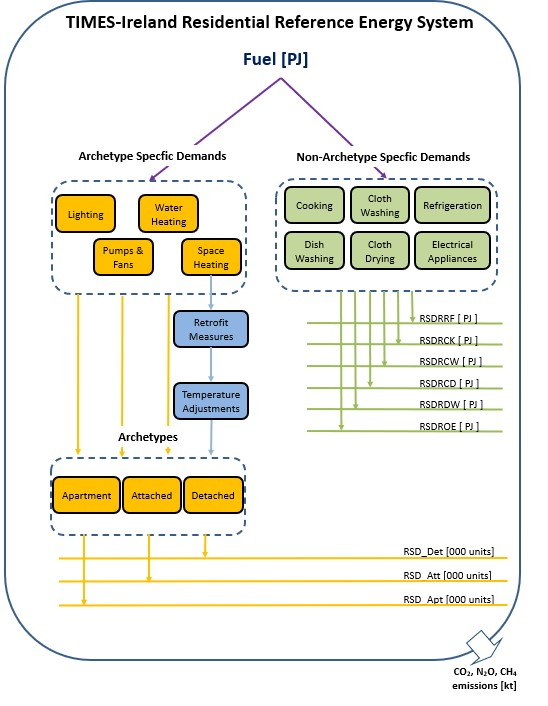
\includegraphics[scale=3.2]{TIM_Residential_RES2.jpg} 
 \caption{Residential Reference Energy System}
 \label{fig:TIM_RES}
\end{figure}

The base-year residential energy demand by fuel is calibrated to the SEAI 2018 Energy Balance \citep{SEAI2019}.

Archetype energy service demands are particularly dependent on the type of building. The four energy service demands which are modelled based on archetype are: space heating, water heating, pump \& fans and lighting. The residential building stock by type is explicitly modelled in TIM in three archetypes: detached, attached and apartments. 

The Archetype energy service demand data are sourced from the SEAI Building Energy Rating (BER) database \citep{SustainableEnergyAuthorityofIreland}, which contains the raw data of 906,048 BER surveys. The BER database was filtered before use, to remove outliers and any nonsensical values. The filters were based upon \citet{Dineen2015}, \citet{Uidhir2020a} and group discussion within a national retrofitting modelling group \citep{NationalRetrofittingModellingGroup} reducing the total records to 815,246.

The filtered BER database is then projected onto the total dwelling stock, using CSO data \citep{CentralStatisticsOffice2020a} , \citep{CentralStatisticsOffice2020b} to calculate the total number BER ratings per archetype in the dwelling stock, as shown in Table \ref{Residential Dwelling Stock}. 

\begin{table}[h!]
 \centering
 \footnotesize
 \caption{Residential Dwelling Stock in 2018}
 \begin{tabular}{ccccc}
 \hline 
 BER Rating & Apartment & Attached & Detached & Total \\ 
 \hline
 A & 9,419 &	15,472 &	20,379 &	45,270 \\
 B1 & 7,459 &	9,538 &	9,434 &	26,431 \\
 B2	& 14,042 &	17,545 &	20,091 &	51,678 \\
 B3 & 19,924 &	49,769 &	53,466 &	123,160 \\
 C & 58,905	& 282,152 &	251,319	& 592,375 \\
 D & 43,739 &	187,627 &	166,668	& 398,034 \\
 E & 25,768 &	101,419 & 	81,397 & 	208,583 \\
 F & 12,331 &	50,124 &	43,241 &	105,696 \\
 G & 15,211 &	52,707 &	78,436 &	146,353 \\
 Total & 206,799 &	766,352	& 724,430 &	1,697,580 \\ \hline 
 \end{tabular}
 \label{Residential Dwelling Stock}
\end{table}

The BER assumes all buildings are heated to between 18\textdegree C (non-living areas, ie. bedroom, bathrooms) to 21\textdegree C (living areas, ie. sitting room, kitchen). This assumption is based upon IS EN 13,790 calculations. To reflect actual energy use based upon internal temperatures in the Irish residential sector, the Archetype Dwelling Energy Model (ArDEM) \citep{Dineen2015} was used to provide simulated annual energy consumption. ArDEM modifies the expected space heating energy consumption of each archetype and BER rating to the actual space heating energy consumption by adjusting internal temperatures in the building stock, a similar approach was used by \citet{Uidhir2020}.

The alternative internal temperatures assumptions in TIM are outlined in Table \ref{Internal Temperature Assumptions}. 

\begin{table}[h!]
 \centering
 \footnotesize
 \caption{Internal Temperature Assumptions}
 \begin{tabular}{ccc}
 \hline 
 BER Rating & Living Area Temperature & Non-living Area Temperature \\
 \hline
 A & 23°C & 20°C \\
 B1 & 21°C & 18°C \\
 B2	& 21°C & 18°C \\
 B3 & 21°C & 18°C \\
 C & 18°C & 15°C \\
 D & 18°C & 15°C \\
 E & 18°C & 15°C \\
 F & 18°C & 15°C \\
 G & 18°C & 13°C \\ \hline
 \end{tabular}
 
 \label{Internal Temperature Assumptions}
\end{table}

% Start this text below the table?? %
After the base year, the change in the number of new dwellings per archetype drives demand, as previously outlined in section \ref{ss:model_proj}. All new dwellings mimic the energy intensity of the average base year A-rated dwelling for that archetype. This is due to directive (EU) 2018/844, which requires all new residential dwellings to equate to at least a A2 BER Rating by 2020. 

The non-archetype energy service demands are: cooking, refrigeration, cloth washing, cloth drying, dish washing and electrical appliances. The non-archetype energy service demands are not dependent on the age, type or BER rating of the future housing type. These demands are projected to grow at the same rate as the growth in the total housing stock. 

Non-Archetype energy demand data was obtained from the SEAI Energy in the Residential Sector Report \citep{SEAISustainableAuthorityofIreland2018}. This data was cross-checked with the JRC-IDEES (Integrated Database of the European Energy System ) database. The process involved cross-checking the share of residential energy service demands in TIM, against a database which had no input in to the model.

\subsubsection{Future technology options}
The TIM residential sector has two main mitigation options - switching heat technologies and fuels, and retrofitting existing dwellings to improve the thermal efficiency and uplift BER ratings. 

While Ireland has ambitious retrofitting targets for 2030, data on the cost and energy savings for retrofitting is limited, particularly for deep retrofits. The expected costs and heat energy saving of retrofitting from one BER rating to another requires further investigation. The retrofit cost data is based upon \citep{AECOMDECLG2013} and \citep{Ali2020} and the expected energy saving is based upon \citep{Collins2017}. For this reason, the model uses a simplistic retrofitting options. There are two options for each archetype: shallow retrofit, which reduces dwelling space heating energy demand by 10-34\% and deep retrofit, which improves space heating energy efficiency by at least 35\%. 

The cost and expected heat energy savings per archetype by BER improvement is outlined in Table \ref{Retrofit Expected Savings}. The model currently implements the weighted average value; fully disaggregated retrofit is planned for implementation in the next model version.

\begin{table}[h!]
 \centering
 \footnotesize
 \caption{Retrofit Cost \& Expected Savings}
 \begin{tabular}{ccccccc}
 \hline
 BER & \multicolumn{2}{c}{Apartment} & \multicolumn{2}{c}{Attached} & \multicolumn{2}{c}{Detached} \\ 
 Rating & Cost & Savings & Cost & Savings & Cost & Savings \\
 \hline
 \multicolumn{7}{c}{Deep Retrofit} \\
 \hline
 C to A & €27,381.6 & 73\% & €30,424 & 73\% & €33,466.4 & 73\% \\
 D to B	& €11,533.5 & 59\% & €12,815 & 60\% & €14,096.5 & 60\% \\
 E to B & €18,273.6 & 70\% & €20,304 & 69\% & €22,334.4 & 69\% \\
 F to B & €19,958.4 & 76\% & €22,176 & 76\% & €24,393.6 & 76\% \\
 G to B & €19,958.4 & 81\% & €22,176 & 81\% & €24,393.6 & 81\% \\
 \hline
 \multicolumn{7}{c}{Shallow Retrofit} \\[0.5ex]
 \hline
 B to A & €18,957.6 & 55\% & €21,064 & 55\% & €23,170.4 & 54\% \\
 C to B & €11,533.5 & 41\% & €9,007.5 & 41\% & €14,096.5 & 40\% \\
 D to C & €7,478.1 & 31\% & €7,536.3 & 32\% & €9,139.9 & 32\% \\
 E to D & €11,848.5 & 26\% & €12,682.5 & 24\% & €14,240.8 & 24\% \\
 F to E & €7,794 & 21\% & €8,660 & 22\% & €9,526 & 21\% \\
 G to F & €2,200 & 20\% & €2,128 & 20\% & €3,200 & 20\% \\ \hline
 \end{tabular}
 
 \label{Retrofit Expected Savings}
\end{table}

The cost and efficiencies of new space heating and water heating technologies available is sourced from the Danish Energy Agency (DEA) database \citep{Energinet2018}. The cost and efficiency of lighting, pumps \& fans and non-archetype demands came from a range of sources including
\citep{SEAISustainableAuthorityofIreland2018} and the ecotopten database \citep{ecotopten}. Ecotopten collects data of household appliances covering around 90\% of the white goods market in the EU.

\subsubsection{User constraints}
\begin{itemize}
 \item The natural gas grid is currently connected to 39\% of apartments, 52\% of attached dwellings and 12\% of detached dwellings. It is assumed that the total share of dwellings connected to the gas grid can grow by 50\% in each category. 
\item Maximum 80\% retrofits in existing buildings.
\item Maximum fuel share in cooking for Gas and LPG is 40\% and 10\% respectively.
\item Maximum 10\% solar input to dual fuel heating technology
\item Maximum 30\% gas input into gas hybrid heating pumps

% THESE ARE NOT ADDED IN THIS ITERATION OF THE MODEL 
%\item maximum decrease constraint in fuel is 10\% / year for electricity, gas, kerosene, LPG and wood. While Solar has a maximum increase constraint of 10\% /year
% (For Future iteration):
%\item It is assumed that any existing dwelling which switches to a heat pump has to undergo a retrofit 
\end{itemize}



\subsection{Industry}
\label{ss:industry}
The industrial sector is modelled using a ``top-down" methodology where energy demand is projected based on an assumed future economic growth. Fourteen subsectors are represented and are based on the SEAI's energy balance \citep{SEAI2019}. Baseline shares of energy carriers in the final energy consumption by subsector are assumed constant into the future and are based on the 2018 values \citep{SEAI2019}. 

%Energy demand for each industrial subsector is projected using Gross Value Added (GVA) for each corresponding NACE category \citep{Yakut2020}. Historical energy consumption is obtained from SEAI's energy balance \citep{SEAI2019}. The total energy demand from industry is projected to increase by 65\% in 2050 from 2018 level. The energy intensity of the industrial sector is expected to decline by 40\% between 2018 and 2050 with a CAGR of -2\%, reflecting historical trends. 

Energy demand for the industrial sector is predicted using Gross Value Added (GVA) per capita for each NACE category and population \citep{Yakut2020}. Historical energy consumption is obtained from SEAI's energy balance \citep{SEAI2019}. The total energy demand from industry is projected to increase by 47\% in 2050 from 2018 level. Cement demand upto 2025 is projected using the Department of finance's stability program update which provides forecasts for the growth in modified investment \cite{April2020}. In 2019, 65\% of the modified investment was in building and construction. A linear regression of the log of the index for output of the cement sector on the log of investment in building and construction at constant price is calculated. This results in an 18.6\% increase in cement demand in 2025 from 2018 level. Beyond 2025, growth in cement demand is assumed to be the same as the growth in GNI*. This leads to a further increase by 17.8\% between 2025 and 2050 at a CAGR of 0.7\%.   The energy intensity of the industrial sector is expected to decline by 46.5\% between 2018 and 2050 with a CAGR of -2\%, reflecting historical trends. 

Fuel switching is the only mitigation option available for combustion emissions from industry in the model. It is controlled through maximum predefined shares which are defined per year and subsector. Table \ref{Maximum fuel switching share in Industry} illustrates assumed maximum fuel switching shares which are possible across all the subsectors. 

\begin{table}[htbp]
\footnotesize
 \centering
 \caption{Maximum fuel switching shares}
 \begin{tabular}{lccc}
 \hline
 Fuel switching option & 2022 & 2030 & 2050 \\
 \hline
 Kerosene to biokerosene & 10\% & 30\% & 100\% \\
 Diesel to biodiesel & 10\% & 30\% & 100\% \\
 Natural gas to biogas & 10\% & 30\% & 100\% \\ 
 Coal and coke to biomass & 8\% & 24\% & 80\% \\ 
 Coal and coke to hydrogen & 2\% & 6\% & 20\% \\ \hline
 \end{tabular}%
 \label{Maximum fuel switching share in Industry}%
\end{table}%

\subsubsection{Process emissions}
Among the industrial processes, the cement industry has the largest share of process emissions, which is accounted for in the model. Historical data of cement production and emissions is obtained from the National Inventory Submissions \citep{NIR2020E91:online}. Process emissions increased by 87\% between 1990 and 2018 with a CAGR of 2.3\%. The kilotonnes of cement required is projected using number of new dwellings and the energy consumption of the corresponding industrial sector in a linear model. The amount of cement needed in 2050 is projected to double relative to 2018 with a CAGR of 2.2\%. The demand for cement is then used to project process emission, which is expected to increase by 96\% between 2018 and 2050 with a CAGR of 2.1\%. 

% Table generated by Excel2LaTeX from sheet 'Sheet1'


%include something on CCS in process emissions
% Table generated by Excel2LaTeX from sheet 'Sheet1'
\begin{table}[htbp]
\footnotesize
 \centering
 \caption{Process emissions}
 \begin{tabular}{lrrrr}
 \hline
 Process emissions (kt/PJ) & \multicolumn{2}{c}{Reference Case} & \multicolumn{2}{c}{with CCS} \\
 & 2018 & 2050 & 2018 & 2050 \\ \hline
 \makecell{Other non-metallic mineral \\ products demand process} & 117 & 155 & 109 & 144 \\ \hline
 \end{tabular}%
 \label{tab:addlabel}%
\end{table}%


\subsection{Services}
\label{ss:services}
The service sector in TIM comprises public and private services. The structure of the sector mostly comes from the Irish TIMES model with an addition of the data centre electricity demand. It includes a representation of the following energy service demands: space heating, space cooling, water heating, cooking, refrigeration, lighting, data centres electricity demand, as well as other energy and electric demand.

%A combination of GVA, population and employment levels is used to project energy demand in the service sector according to the NACE categories (except for data centres) available in the SEAI's energy balance \citep{SEAI2019}. Energy demand from commercial and public services is expected to increase by 86\% in 2050. 

Future fuel switching and efficiency options in the Services sector are modelled in a top-down fashion given a lack of sufficient building-level data to enable a bottom-up analysis. This is an area identified as a priority area for future model development. 

The end-use demand services in the service sector include million meter square of area for public and private sector buildings, data centre demand and public lighting units. The area is projected assuming the same growth as in GNI*. The total area is projected to increase by 61.8\% by 2050 from 2018 level with a CAGR of 1.5\%. 

Electricity demand for data centres is obtained from EirGrid, i.e. their ``steady evolution" scenario. \citep{EirGridT57:online}. The electricity demand for data centres is expected to increase by 6 times in 2030 from 2018 level. We assume no growth in data centre demand after 2030 since permission requests for new/expanding existing capacities are not available yet. Further, post-2030 demand is even more uncertain given (i) the potential for exponential data usage growth and further data centres applications vs (ii) technology improvements and whether data centres fully utilise their contracted import capacity.  

Public lighting units are projected based on the Project Ireland 2040, whereby five major cities of Ireland, Dublin, Cork, Limerick, Galway and Waterford are expected to grow by 50\% in 2040 \citep{GovernmentofIreland2018}. This results in a 12.5\% increase in public lighting units in Ireland by 2040 from 2018 level, with a CAGR of 1\%. Beyond 2040, the units are projected to increase by 1\% per annum until 2050.

\subsection{Agriculture}
\label{ss:agriculture}
The current version of the agriculture sector in TIM comes from the Irish TIMES model and is documented in \citet{Chiodi2016}. It includes representation of 12 energy service demands; half of them belong to the livestock and half to the tillage sector. Land availability and water consumption are explicitly represented and accounted for in the sector, however no specific constraints are set. Future energy service demands in the agriculture sector are assumed to be unchanged from the 2018 level.

%\section{Model application}
%\label{s:model_appl}


\section{Discussion \& conclusion}
\label{s:discussion}
This section discusses the strengths, limitations and development priorities for the TIMES-Ireland model, using the framework proposed by \citet{Pye2020} and \citet{DeCarolis2017}, which outline best practice for ESOM development and priorities for new developments and applications of ESOMs for deep decarbonisation challenges.

\subsection{Analytical advancements}
The following is a summary of the main analytical advancements of TIM, explained in more detail throughout the text. 
\begin{itemize}
\item The power sector has a flexible time-slice configuration with resolution possible up to the hourly level, which is necessary to model the power system under very high shares of variable renewables in deep decarbonisation scenarios, including power storage. 
\item The power sector also makes use of new TIMES features, modelling dispatch, unit commitment and capacity expansion.
\item The model as a whole has been developed with flexible regional definitions, with parts of the transport and power sectors detailed at the county level. 
\item Energy service demands are driven by a consistent set of population and macro-economic indicators, consistent with a national CGE model, and also disaggregated in sufficient detail to allow alternative demand scenarios, such as transport mode shifting, lower housing demand requirements etc.
\item The development process strives to achieve best practice in software development, including version control, transparency (with open source and open data), quality assurance, documentation and wide stakeholder consultation. 
\end{itemize}

\subsection{Modelling for policy insight}
The main purpose of the model is to meet the policy need to inform detailed sectoral pathways which can meet very ambitious decarbonisation targets. This subsection discusses TIM's strengths and weaknesses in this regard. 

Firstly, the integrated whole system approach offer ``macro systems" perspective .. The temporal and spatial flexibility resolves the tension between the requirements for granularity for certain model functionalities, and the requirement for data and model tractability, and fast solving speed. Integration with key national data sources and other models is a further strength of TIM. 

Secondly, an appropriately wide mitigation option space is required to meet deep decarbonisation challenges. Strengths of TIM include the rich depiction of important demand sectors, namely transport and residential, which are characterised to enable scenario variants of alternative demands. For example, splitting passenger transport demand into long-, medium- and short-distance demand allows for switching to active and public transport demands . Similarly, the archetypal model underpinning the residential sector allows for lowering building floor area demand and internal temperatures, which can be key scenario variants. These scenario variants are endogenous, though there is increasing literature on endogenising behaviour in TIMES models. Several options for shifting to more efficient uses of energy, for example, are endogenous. However, the aggregate nature of the Industry and Services sectors limits the potential analysis of demand reduction in these sectors and is an area of future model development priority.

Another area for future model improvements is to explore carbon dioxide removal (CDR) options in more detail. At the global level, modelled pathways meeting the Paris Agreement rely on large-scale deployment of CDR options including biomass with carbon capture and storage (BECCS) \citep{IPCC2018}. BECCS is currently modelled within TIM, but options like Direct Air Capture (DAC)\citep{Realmonte2019} are currently not.

Another limitation of TIM is the sole focus on energy and process emissions. Agriculture and land-use are very significant emitters in Ireland, and future energy system decarbonisation trajectories will require a focus on the overlaps with other emitters. This is required firstly to understand bioenergy and waste potentials, and to take into account future gains from the circular economy, and also competition between energy crops, agriculture and reforestation.

A focus on the practice of model development and application is key. Robust quantitative analysis and information is an important ingredient in the energy and climate policy making process. But energy modelling should support the policy making process rather than determine its contents. This means the interface between energy modelling and the policy making process should be an iterative one that incorporates regular review and feedback as new issues and questions emerge \citep{strachan2016reinventing}. TIM has been developed with the aims of openness and transparency, quality assurance and best practice in software development, and iterative engagement with key stakeholders to feed in sectoral and industry expertise, and to be able reflect policy and societal factors. Any model built to inform policy should be open to deep scrutiny early and throughout the process. It also requires capacity-development among the ``consumers" of model outputs to ensure that results are interpreted, communicated and applied appropriately.

It is also important to communicate what the model can and can't do. For example, while TIM is a ''cost-optimal" model, it does not capture many of the societal costs or benefits that the energy system imposes. For example, higher renewable energy shares may represent a higher overall investment and operation cost over the project lifetime, these may offer significant societal benefits in terms of lower air pollution, reducing the fossil fuel import bill and providing high-quality employment. Similarly, the distributional effects of the costs are not captured in the model, therefore considerations of a ''just transition" are a challenge within TIM currently. 


\subsection{Future improvements}
TIM will undergo continuous and iterative improvements and developments. In the near-term, the following is the priority list for future development:
\begin{itemize}
 \item Modelling gas supply at hourly resolution - currently modelled at a seasonal level, which may unintentionally allow for energy storage capacity.
 \item Similarly, electricity interconnectors with the UK and France can be modelled at the same time resolution as the power sector, taking into account capacity constraints on top of annual trade constraints.
 \item Modelling hydrogen production routes other than from renewables (green hydrogen), such as blue, brown and grey hydrogen production options. 
 \item A review and update of bioenergy conversion options, including an update of domestic bioenergy potentials. 
 \item A review and update of future low-carbon technology costs.
 \item Developing further the Agri-TIMES module, first developed by \citet{Chiodi2016}, in order to model agriculture, livestock and land-use emissions and mitigation options explicitly, including competition for land-use.
 \item A more detailed bottom-up focus on the Industry and Services sectors, which are currently modelled in an aggregated top-down fashion. 
 \item Developing a ``Business as usual"/``With existing policy measures" case, which includes current policies and measures and hurdle rates to represent end-use technology uptake.
\end{itemize}


\conclusions  %% \conclusions[modified heading if necessary]
\label{s:conclusion}
This paper presents the TIMES-Ireland Model (TIM), an energy systems optimisation model which is a significant step forward both in terms of analytical heft, open and best-practice development approach and in its contribution to national evidence-based policy development. TIM has been developed to help inform very ambitious decarbonisation objectives and to inform future carbon budgets, on the path to net-zero GHG emissions by 2050. 

The model was developed from the legacy model, Irish TIMES, which has had a long history of contributing the the evidence base for Irish energy policy and for pushing the state-of-the-art in ESOM development. TIM also benefits from ongoing collaborations and interactions with other national models and data sources, including LEAP-Ireland, the ESRI's I3E model and SEAI databases. The model also benefits from the continuous development of the TIMES model generator within the ETSAP community.

Continuous, iterative and open model development is essential to ensure that the model remains fit-for-purpose and state-of-the-art. The model has been built with these future calibrations and improvements in mind, with clear open documentation and development protocol to allow for ongoing improvements and updates, to better enable the Irish energy system to achieve the goal of carbon neutrality. 

%% The following commands are for the statements about the availability of data sets and/or software code corresponding to the manuscript.
%% It is strongly recommended to make use of these sections in case data sets and/or software code have been part of your research the article is based on.

%%\codeavailability{TEXT} %% use this section when having only software code available


\dataavailability{
TIMES code is available [zenodo doi]...
Data will be available through github and published in zenodo.} %% use this section when having only data sets available


%%\codedataavailability{TEXT} %% use this section when having data sets and software code available


%%\sampleavailability{TEXT} %% use this section when having geoscientific samples available


%%\videosupplement{TEXT} %% use this section when having video supplements available



%% The Appendices part is started with the command \appendix;
%% appendix sections are then done as normal sections
\clearpage


\appendix 
\section{Supplementary techno-economic assumptions}
\label{s:Appendix-data}


\begin{table}[!htbp]
\footnotesize
\caption{Import Fossil fuel commodity prices}
\scalebox{0.9}{
\begin{tabular}{llllllll}
\hline 
Technology Description & 2018 & 2019 & 2025 & 2030 & 2035 & 2040 & *Source/Ratio \\

 & €/GJ & €/GJ & €/GJ & €/GJ & €/GJ & €/GJ & \\
\hline 
Crude Oil & 10.1 & 9.9 & 11.1 & 11.9 & 12.7 & 13.3 & WEO2019/2020 \\
Natural Gas - UK & 6.1 & 5.7 & 6.2 & 9.4 & 11.0 & 12.9 & WEO2019/2020 \\
Hard Coal / Antracite & 1.9 & 1.3 & 1.4 & 1.7 & 1.9 & 2.1 & WEO2019/2020 \\
Bituminous Coal & 1.8 & 1.2 & 1.3 & 1.6 & 1.8 & 2.0 & 0.95 \\
Coke Coal & 2.4 & 1.7 & 1.8 & 2.2 & 2.4 & 2.6 & 1.27 \\
Lignite / Brown Coal & 1.6 & 1.1 & 1.2 & 1.5 & 1.6 & 1.8 & 0.88 \\
Liquefied Natural Gas & 6.5 & 6.1 & 6.6 & 10.0 & 11.7 & 13.8 & 1.07 \\
Diesel Oil & 15.4 & 15.1 & 17.0 & 18.2 & 19.4 & 20.3 & 1.53 \\
Gasoline & 16.6 & 16.2 & 18.3 & 19.6 & 20.9 & 21.9 & 1.65 \\
Heavy Fuel Oil & 8.2 & 8.0 & 9.0 & 9.6 & 10.3 & 10.8 & 0.81 \\
Kerosene & 16.6 & 16.2 & 18.3 & 19.6 & 20.9 & 21.9 & 1.65 \\
Liquefied Petroleum Gas & 13.0 & 12.8 & 14.4 & 15.4 & 16.4 & 17.2 & 1.29 \\
Petroleum Coke & 16.6 & 16.2 & 18.3 & 19.6 & 20.9 & 21.9 & 1.65 \\
Uranium & & & & & & & \\
Oil for Non-Energy uses & 10.1 & 9.9 & 11.1 & 11.9 & 12.7 & 13.3 & \\ \hline 
\end{tabular}
}
\label{import-fuel-prices}
\end{table}


\begin{table}[!htbp]
\footnotesize
\caption{Import bioenergy commodity prices}
\scalebox{0.9}{
\begin{tabular}{lllllll}
\hline
Bioenergy Import Costs & 2015 & 2020 & 2025 & 2030 & 2040 & 2050 \\

Technology Description & €/GJ & €/GJ & €/GJ & €/GJ & €/GJ & €/GJ \\
\hline 
Import of Ethanol 1st generation - Step 1 & 18.18 & 17.58 & 16.60 & 15.88 & & \\
Import of Ethanol 1st generation - Step 2 & 18.92 & 19.08 & 18.92 & 19.13 & 20.39 & 21.40 \\
Import of Ethanol 1st generation - Step 3 & 19.68 & 20.68 & 21.76 & 23.55 & 25.10 & 26.34 \\
Import of Ethanol 1st generation - Step 4 & 20.64 & 22.71 & 25.17 & 28.76 & 30.65 & 32.16 \\
Import of Biodiesel 1st generation - Step 1 & 31.36 & 33.18 & 31.86 & 31.34 & & \\
Import of Biodiesel 1st generation - Step 2 & 32.65 & 35.83 & 35.97 & 37.02 & 39.46 & 41.41 \\
Import of Biodiesel 1st generation - Step 3 & 33.92 & 38.33 & 40.46 & 43.76 & 46.64 & 48.94 \\
Import of Biodiesel 1st generation - Step 4 & 35.54 & 41.92 & 46.53 & 52.83 & 56.31 & 59.09 \\
Import of Wood Pellets - Step 1 & 10.65 & 8.50 & 7.28 & 6.95 & & \\
Import of Wood Pellets - Step 2 & 11.03 & 9.05 & 8.07 & 7.91 & & \\
Import of Wood Pellets - Step 3 & 12.28 & 10.10 & 8.93 & 8.77 & & \\
Import of Wood Pellets - Step 4 & 12.78 & 10.80 & 9.98 & 10.06 & & \\
Import of Wood Chip - Step 1 & 5.21 & 4.16 & 3.56 & 3.39 & & \\
Import of Wood Chip - Step 2 & 5.40 & 4.42 & 3.94 & 3.87 & & \\
Import of Wood Chip - Step 3 & 6.14 & 5.04 & 4.47 & 4.37 & & \\
Import of Wood Chip - Step 4 & 6.38 & 5.40 & 4.99 & 5.04 & & \\ \hline 
\end{tabular}
}
\label{import-bio-prices}
\end{table}	


\begin{table}[!htbp]
\footnotesize
\caption{Import bioenergy delivery costs}
\scalebox{0.9}{
\begin{tabular}{lccccc}
\hline
Bioenergy Import Delivery Costs & \multicolumn{1}{l}{2020} & \multicolumn{1}{l}{2030} & \multicolumn{1}{l}{2040} & \multicolumn{1}{l}{2050} & \multicolumn{1}{l}{Notes} \\

Technology Description & \multicolumn{1}{l}{€/GJ} & \multicolumn{1}{l}{€/GJ} & \multicolumn{1}{l}{€/GJ} & \multicolumn{1}{l}{€/GJ} & \multicolumn{1}{l}{} \\
\hline 
Import of Wood Pellets - Step 1 & 4.32 & 4.45 & 4.59 & 4.69 & \\
Import of Wood Pellets - Step 2 & 4.32 & 4.45 & 4.59 & 4.69 & \\
Import of Wood Pellets - Step 3 & 4.32 & 4.45 & 4.59 & 4.69 & \\
Import of Wood Pellets - Step 4 & 4.32 & 4.45 & 4.59 & 4.69 & \\
Import of Wood Chip - Step 1 & 4.32 & 4.45 & 4.59 & 4.69 & \\
Import of Wood Chip - Step 2 & 4.32 & 4.45 & 4.59 & 4.69 & \\
Import of Wood Chip - Step 3 & 4.32 & 4.45 & 4.59 & 4.69 & \\
Import of Wood Chip - Step 4 & 4.32 & 4.45 & 4.59 & 4.69 & \\ \hline 
\end{tabular}
}
\label{import-bio-delivery-costs}
\end{table}

\begin{table}[!htbp]
\footnotesize
\caption{Import bioenergy potentials}
\scalebox{0.9}{
\begin{tabular}{lllllllll}
\hline 
Imported Bioenergy potentials (PJ) & 2018 & 2020 & 2025 & 2030 & 2035 & 2040 & 2045 & 2050 \\

Technology Description & PJ & PJ & PJ & PJ & PJ & PJ & PJ & PJ \\
\hline 
Import of Ethanol 1st generation - Step 1 & 1.0 & 1.0 & 1.0 & 1.0 & 1.0 & 1.0 & 1.0 & 1.0 \\
Import of Ethanol 1st generation - Step 2 & 0.0 & 1.9 & 1.9 & 1.9 & 1.9 & 1.9 & 1.9 & 1.9 \\
Import of Ethanol 1st generation - Step 3 & 0.0 & 3.8 & 3.8 & 3.8 & 3.8 & 3.8 & 3.8 & 3.8 \\
Import of Ethanol 1st generation - Step 4 & 0.0 & 27.1 & 27.1 & 27.1 & 27.1 & 27.1 & 27.1 & 27.1 \\
 & & & & & & & & \\
Import of Biodiesel 1st generation - Step 1 & 4.4 & 4.4 & 4.4 & 4.4 & 4.4 & 4.4 & 4.4 & 4.4 \\
Import of Biodiesel 1st generation - Step 2 & 0.0 & 8.7 & 8.7 & 8.7 & 8.7 & 8.7 & 8.7 & 8.7 \\
Import of Biodiesel 1st generation - Step 3 & 0.0 & 17.4 & 17.4 & 17.4 & 17.4 & 17.4 & 17.4 & 17.4 \\
Import of Biodiesel 1st generation - Step 4 & 0.0 & 72.2 & 72.2 & 72.2 & 72.2 & 72.2 & 72.2 & 72.2 \\
 & & & & & & & & \\
Import of Wood Pellets - Step 1 & 0.7 & 0.7 & 0.7 & 0.7 & 0.7 & 0.7 & 0.7 & 0.7 \\
Import of Wood Pellets - Step 2 & 0.0 & 1.4 & 1.4 & 1.4 & 1.4 & 1.4 & 1.4 & 1.4 \\
Import of Wood Pellets - Step 3 & 0.0 & 2.7 & 2.7 & 2.7 & 2.7 & 2.7 & 2.7 & 2.7 \\
Import of Wood Pellets - Step 4 & 0.0 & 105.4 & 105.4 & 105.4 & 105.4 & 105.4 & 105.4 & 105.4 \\
 & & & & & & & & \\
Import of Wood Chip - Step 1 & 0.3 & 0.3 & 0.3 & 0.3 & 0.3 & 0.3 & 0.3 & 0.3 \\
Import of Wood Chip - Step 2 & 0.0 & 0.6 & 0.6 & 0.6 & 0.6 & 0.6 & 0.6 & 0.6 \\
Import of Wood Chip - Step 3 & 0.0 & 1.2 & 1.2 & 1.2 & 1.2 & 1.2 & 1.2 & 1.2 \\
Import of Wood Chip - Step 4 & 0.0 & 34.7 & 34.7 & 34.7 & 34.7 & 34.7 & 34.7 & 34.7 \\ \hline
\end{tabular}
}
\label{bioenergy-potentials}
\end{table}

\begin{center}
\footnotesize
\begin{longtable}{p{15em}lllll}
\caption{Base year generation units} \\
\hline
Technology description & Efficiency & Availability & Life & Start & Capacity \\
Units & & & Years & Year & GW \\
\hline \endfirsthead
\multicolumn{6}{c}%
{{\bfseries \tablename\ \thetable{} -- continued from previous page}} \\
\hline
Technology description & Efficiency & Availability & Life & Start & Capacity \\
Units & & & Years & Year & GW \\
\hline \endhead
\hline \endfoot
PWR Renewable: Hydropower dam and reservoir HYD Existing Ardnacrusha 1 & 1.00 & 0.45 & 150 & 1929 & 0.02 \\
PWR Renewable: Hydropower dam and reservoir HYD Existing Ardnacrusha 2 & 1.00 & 0.45 & 150 & 1929 & 0.02 \\
PWR Renewable: Hydropower dam and reservoir HYD Existing Ardnacrusha 3 & 1.00 & 0.44 & 150 & 1929 & 0.02 \\
PWR Renewable: Hydropower dam and reservoir HYD Existing Ardnacrusha 4 & 1.00 & 0.45 & 150 & 1929 & 0.02 \\
PWR Thermal Power Plant: Combined cycle gas turbine GAS Existing Aghada CCGT & 0.70 & 0.90 & 30 & 2010 & 0.43 \\
PWR Thermal Power Plant: Open cycle gas turbine GAS Existing Aghada CT 1 & 0.42 & 0.95 & 43 & 1980 & 0.09 \\
PWR Thermal Power Plant: Open cycle gas turbine GAS Existing Aghada CT 2 & 0.42 & 0.95 & 44 & 1980 & 0.09 \\
PWR Thermal Power Plant: Open cycle gas turbine GAS Existing Aghada CT 4 & 0.42 & 0.95 & 44 & 1980 & 0.09 \\
PWR Thermal Power Plant: Combined cycle gas turbine GAS Existing Ballylumford CCGT Unit 10 & 0.60 & 0.90 & 35 & 2003 & 0.10 \\
PWR Thermal Power Plant: Combined cycle gas turbine GAS Existing Ballylumford CCGT Unit 31 & 0.63 & 0.90 & 35 & 2003 & 0.25 \\
PWR Thermal Power Plant: Combined cycle gas turbine GAS Existing Ballylumford CCGT Unit 32 & 0.63 & 0.90 & 35 & 2003 & 0.25 \\
PWR Thermal Power Plant: Open cycle gas turbine DIS Existing Ballylumford GT1 & 0.33 & 0.95 & 50 & 1976 & 0.06 \\
PWR Thermal Power Plant: Open cycle gas turbine DIS Existing Ballylumford GT2 & 0.33 & 0.95 & 50 & 1976 & 0.06 \\
PWR Thermal Power Plant: Open cycle gas turbine DIS Existing Coolkeeragh OCGT & 0.33 & 0.95 & 35 & 2005 & 0.05 \\
PWR Thermal Power Plant: Open cycle gas turbine GAS Existing Contour Global Agg Unit & 0.45 & 0.95 & 35 & 2010 & 0.01 \\
PWR Thermal Power Plant: Combined cycle gas turbine GAS Existing Coolkeeragh CCGT & 0.68 & 0.90 & 35 & 2005 & 0.41 \\
PWR Thermal Power Plant: Combined cycle gas turbine GAS Existing Dublin Bay CCGT & 0.68 & 0.90 & 30 & 2002 & 0.41 \\
PWR Thermal Power Plant: Steam turbine PEA Existing Edenderry & 0.49 & 0.90 & 23 & 2000 & 0.12 \\
PWR Thermal Power Plant: Open cycle gas turbine DIS Existing Cushaling & 0.38 & 0.95 & 30 & 2010 & 0.06 \\
PWR Thermal Power Plant: Open cycle gas turbine DIS Existing Cushaling & 0.38 & 0.95 & 30 & 2010 & 0.06 \\
PWR Renewable: Hydropower dam and reservoir HYD Existing Erne 1 & 1.00 & 0.47 & 150 & 1950 & 0.01 \\
PWR Renewable: Hydropower dam and reservoir HYD Existing Erne 2 & 1.00 & 0.43 & 150 & 1950 & 0.01 \\
PWR Renewable: Hydropower dam and reservoir HYD Existing Erne 3 & 1.00 & 0.47 & 150 & 1950 & 0.02 \\
PWR Renewable: Hydropower dam and reservoir HYD Existing Erne 4 & 1.00 & 0.40 & 150 & 1950 & 0.02 \\
PWR Thermal Power Plant: Combined cycle gas turbine GAS Existing Great Island CCGT & 0.71 & 0.90 & 35 & 2014 & 0.43 \\
PWR Thermal Power Plant: Combined cycle gas turbine GAS Existing Huntstown Phase II & 0.75 & 0.90 & 30 & 2007 & 0.41 \\
PWR Thermal Power Plant: Combined cycle gas turbine GAS Existing Huntstown & 0.70 & 0.90 & 30 & 2002 & 0.34 \\
PWR Thermal Power Plant: Combined cycle gas turbine DIS Existing iPower AGU & 0.34 & 0.90 & 35 & 2011 & 0.00 \\
PWR Thermal Power Plant: Steam turbine COA Existing Kilroot Unit 1 FGD & 0.18 & 0.90 & 50 & 1981 & 0.20 \\
PWR Thermal Power Plant: Steam turbine COA Existing Kilroot Unit 2 FGD & 0.18 & 0.90 & 50 & 1982 & 0.20 \\
PWR Thermal Power Plant: Open cycle gas turbine DIS Existing Kilroot GT1 & 0.33 & 0.95 & 35 & 2009 & 0.03 \\
PWR Thermal Power Plant: Open cycle gas turbine DIS Existing Kilroot GT2 & 0.33 & 0.95 & 35 & 2009 & 0.03 \\
PWR Thermal Power Plant: Open cycle gas turbine DIS Existing Kilroot GT3 & 0.39 & 0.95 & 35 & 2009 & 0.04 \\
PWR Thermal Power Plant: Open cycle gas turbine DIS Existing Kilroot GT4 & 0.39 & 0.95 & 35 & 2009 & 0.04 \\
PWR Renewable: Hydropower dam and reservoir HYD Existing Lee 1 & 1.00 & 0.33 & 150 & 1957 & 0.02 \\
PWR Renewable: Hydropower dam and reservoir HYD Existing Lee 2 & 1.00 & 0.33 & 150 & 1957 & 0.00 \\
PWR Renewable: Hydropower dam and reservoir HYD Existing Lee 3 & 1.00 & 0.33 & 150 & 1957 & 0.01 \\
PWR Renewable: Hydropower dam and reservoir HYD Existing Liffey 1 & 1.00 & 0.11 & 150 & 1938 & 0.02 \\
PWR Renewable: Hydropower dam and reservoir HYD Existing Liffey 2 & 1.00 & 0.10 & 150 & 1938 & 0.02 \\
PWR Renewable: Hydropower dam and reservoir HYD Existing Liffey 4 & 1.00 & 0.11 & 150 & 1938 & 0.00 \\
PWR Renewable: Hydropower dam and reservoir HYD Existing Liffey 5 & 1.00 & 0.11 & 150 & 1938 & 0.00 \\
PWR Thermal Power Plant: Steam turbine PEA Existing Lough Ree & 0.41 & 0.90 & 16 & 2004 & 0.09 \\
PWR Thermal Power Plant: Steam turbine COA Existing Moneypoint 1 & 0.34 & 0.90 & 38 & 1987 & 0.29 \\
PWR Thermal Power Plant: Steam turbine COA Existing Moneypoint 2 & 0.34 & 0.90 & 38 & 1987 & 0.29 \\
PWR Thermal Power Plant: Steam turbine COA Existing Moneypoint 3 & 0.34 & 0.90 & 38 & 1987 & 0.29 \\
PWR Thermal Power Plant: Open cycle gas turbine GAS Existing North Wall 5 & 0.41 & 0.95 & 30 & 2012 & 0.10 \\
PWR Thermal Power Plant: Combined cycle gas turbine GAS Existing Poolbeg C\_A & 0.58 & 0.90 & 30 & 2000 & 0.26 \\
PWR Thermal Power Plant: Combined cycle gas turbine GAS Existing Poolbeg C\_B & 0.58 & 0.90 & 30 & 2000 & 0.26 \\
PWR Thermal Power Plant: Open cycle gas turbine DIS Existing Rhode 1 & 0.37 & 0.95 & 30 & 2004 & 0.05 \\
PWR Thermal Power Plant: Open cycle gas turbine DIS Existing Rhode 2 & 0.37 & 0.95 & 30 & 2004 & 0.05 \\
PWR Thermal Power Plant: Open cycle gas turbine GAS Existing Sealrock 3 (Aughinish CHP) & 0.72 & 0.93 & 35 & 2005 & 0.08 \\
PWR Thermal Power Plant: Open cycle gas turbine GAS Existing Sealrock 4 (Aughinish CHP) & 0.72 & 0.93 & 35 & 2005 & 0.08 \\
PWR Thermal Power Plant: Steam turbine HFO Existing Tarbert Unit 1 & 0.31 & 0.95 & 54 & 1969 & 0.05 \\
PWR Thermal Power Plant: Steam turbine HFO Existing Tarbert Unit 2 & 0.31 & 0.95 & 54 & 1969 & 0.05 \\
PWR Thermal Power Plant: Steam turbine HFO Existing Tarbert Unit 3 & 0.42 & 0.95 & 54 & 1969 & 0.24 \\
PWR Thermal Power Plant: Steam turbine HFO Existing Tarbert Unit 4 & 0.40 & 0.95 & 54 & 1969 & 0.24 \\
PWR Thermal Power Plant: Open cycle gas turbine DIS Existing Tawnaghmore 1 & 0.38 & 0.95 & 30 & 2003 & 0.05 \\
PWR Thermal Power Plant: Open cycle gas turbine DIS Existing Tawnaghmore 3 & 0.38 & 0.95 & 30 & 2003 & 0.05 \\
PWR Thermal Power Plant: Combined cycle gas turbine GAS Existing Tynagh & 0.68 & 0.90 & 30 & 2006 & 0.40 \\
PWR Thermal Power Plant: Combined cycle gas turbine GAS Existing Whitegate & 0.75 & 0.90 & 30 & 2010 & 0.45 \\
PWR Thermal Power Plant: Steam turbine PEA Existing West Offaly & 0.42 & 0.90 & 15 & 2005 & 0.14 \\
PWR Storage: Pumped Storage HYD Existing Turlough Hill 1 & 0.75 & 0.16 & 150 & & 0.07 \\
PWR Storage: Pumped Storage HYD Existing Turlough Hill 2 & 0.75 & 0.16 & 150 & & 0.07 \\
PWR Storage: Pumped Storage HYD Existing Turlough Hill 3 & 0.75 & 0.16 & 150 & & 0.07 \\
PWR Storage: Pumped Storage HYD Existing Turlough Hill 4 & 0.75 & 0.16 & 150 & & 0.07 \\ \hline

\label{base year generation units}
\end{longtable}
\end{center}

\begin{table}[!htbp]
 \centering
 \footnotesize
 \caption{Residential Heating Cost \& Efficiency. Note: it is assumed a water heaters are 30\% less efficient than space heaters. The costs shown are for space heaters only.}
 \begin{tabular}{cccccccccc}
 \hline
 \multicolumn{2}{c}{Description} & \multicolumn{2}{c}{2020} & \multicolumn{2}{c}{2030} & \multicolumn{2}{c}{2040} & \multicolumn{2}{c}{2050} \\
 
 Archetype & Technology & k€ & $\eta$ & k€ & $\eta$ & k€ & $\eta$ & k€ & $\eta$ \\
 \hline
 \multirow{3}{*}{Apartment}&Gas Boiler & 2.79 & 81\% & 2.79 & 81\% & 2.79 & 81\% & 2.79 & 81\% \\
 & Oil Boiler & 3.63 & 81\% & 3.63 & 81\% & 3.63 & 81\% & 3.63 & 81\% \\
 & Heat Pump & 7.5 & 307\% & 6.83 & 338\% & 6.21 & 379\% & 6.15 & 409\% \\
 \hline
 \multirow{3}{*}{Attached}&Gas Boiler & 3.25 & 82\% & 3.25 & 82\% & 3.25 & 82\% & 3.25 & 82\% \\
 & Oil Boiler & 4.23 & 82\% & 4.23 & 82\% & 4.23 & 82\% & 4.23 & 82\% \\
 & Heat Pump & 8.53 & 312\% & 7.76 & 343\% & 7.06 & 384\% & 6.99 & 415\% \\
 \hline
 \multirow{3}{*}{Detached}&Gas Boiler & 3.53 & 83\% & 3.53 & 83\% & 3.53 & 83\% & 3.53 & 83\% \\
 & Oil Boiler & 4.58 & 82\% & 4.58 & 82\% & 4.58 & 82\% & 4.58 & 82\% \\
 & Heat Pump & 9.85 & 309\% & 8.96 & 340\% & 8.15 & 381\% & 8.07 & 412\% \\ \hline
 \end{tabular}
 
 \label{Residential Heating Cost & Efficiency}
\end{table}


\begin{table}[!htbp]
 \centering
 \begin{threeparttable}
 \footnotesize
 \caption{Techno-economic characteristics of passenger transport vehicles}
 \begin{tabular}{lrrrrc}
 \hline
 Technology (fuel) & \multicolumn{2}{c}{\makecell{Fuel economy \\ (million vkm/PJ)}} & \multicolumn{2}{c}{\makecell{Purchase price\tnote{a} \\(\euro{2018})}} & \multicolumn{1}{p{8.215em}}{\makecell{Annual \\ maintenance \\ cost (\euro{2018}) }} \\
 & 2018 & 2050 & 2018 & 2050 & \\ \hline
 \textbf{Light-duty vehicles} & & & & & \\
 ICE (Gasoline) & 413 & 413 & 20,290 & 20,290 & 1,015 \\
 ICE (E85) & 389 & 418 & 20,290 & 20,290 & 1,015 \\
 ICE (Diesel/B20) & 573 & 615 & 21,832 & 21,832 & 1,092 \\
 ICE (B100) & 556 & 596 & 21,832 & 21,832 & 1,092 \\
 ICE (Dual-fuel) & 413 & 413 & 20,290 & 20,290 & 1,015 \\
 ICE (CNG/BioCNG) & 413 & 443 & 24,631 & 24,631 & 1,232 \\
 HEV (Gasoline) & 556 & 596 & 23,752 & 22,769 & 1,188 \\
 HEV (Diesel) & 719 & 772 & 25,646 & 24,569 & 1,282 \\
 PHEV (Gasolone, Electricity) & 940 & 1,081 & 30,950 & 25,371 & 1,547 \\
 PHEV (Diesel, Electricity) & 1,216 & 1,398 & 33,424 & 27,377 & 1,671 \\
 BEV (Electricity) & 1,623 & 1,886 & 32,971 & 24,646 & 1,649 \\
 FCV (Hydrogen) & 882 & 1,012 & 60,819 & 24,796 & 3,041 \\
 \textbf{Buses} & & & & & \\
 ICE (Diesel) & 106 & 114 & 109,959 & 113,565 & 5,498 \\
 ICE (B100) & 106 & 114 & 109,959 & 113,565 & 5,498 \\
 ICE (CNG/BioCNG) & 101 & 108 & 109,959 & 113,565 & 5,498 \\
 BEV (electricity) & 337 & 391 & 397,219 & 130,000 & 19,861 \\
 FCV (hydrogen) & 192 & 236 & 397,219 & 130,689 & 19,861 \\
 \textbf{Train} & & & & & \\
 Light train BEV (Electricity) & 21 & 21 & 231,583 & 231,583 & 11,579 \\
 Heavy train BEV (Electricity) & 21 & 21 & 935,522 & 935,522 & 46,776 \\
 Heavy train ICE (Diesel) & 8 & 8 & 989,272 & 989,272 & 49,464 \\ \hline
 \end{tabular}
 \begin{tablenotes}
 \item[a] The values exclude taxes and subsidies
 \end{tablenotes}
 \end{threeparttable}
 \label{vehicle-purchase}
 \end{table}


\clearpage

\noappendix    %% use this to mark the end of the appendix section. Otherwise the figures might be numbered incorrectly (e.g. 10 instead of 1).

%% Regarding figures and tables in appendices, the following two options are possible depending on your general handling of figures and tables in the manuscript environment:

%% Option 1: If you sorted all figures and tables into the sections of the text, please also sort the appendix figures and appendix tables into the respective appendix sections.
%% They will be correctly named automatically.

%% Option 2: If you put all figures after the reference list, please insert appendix tables and figures after the normal tables and figures.
%% To rename them correctly to A1, A2, etc., please add the following commands in front of them:

%%\appendixfigures  %% needs to be added in front of appendix figures

%%\appendixtables   %% needs to be added in front of appendix tables

%% Please add \clearpage between each table and/or figure. Further guidelines on figures and tables can be found below.

\authorcontribution{TEXT} %% this section is mandatory

\competinginterests{TEXT} %% this section is mandatory even if you declare that no competing interests are present

\disclaimer{TEXT} %% optional section

\begin{acknowledgements}
This work is being undertaken as part of a number of research projects undertaken at the SFI MaREI Centre at University College Cork, including CAPACITY, funded by the Department of Environment, Climate and Communications and the SFI-funded CHIMERA project\footnote{CHIMERA is supported by a research grant from Science Foundation Ireland (SFI) and the National Natural Science Foundation of China (NSFC) under the SFI-NSFC Partnership Programme, grant no. 17/NSFC/5181 and supported by MaREI, the SFI Research Centre for Energy, Climate, and Marine [Grant No: 12/RC/2302\_P2], https://www.marei.ie/project/chimera/}.

The authors wish to acknowledge the contribution of the following people: Alessandro Chiodi, Paul Deane, Maurizio Gargiulo, Gerald Lyons, Brian O'Gallachoir, Fionn Rogan, Andrew Smith.
\end{acknowledgements}


%% REFERENCES

%% The reference list is compiled as follows:

%%\begin{thebibliography}{}

%%\bibitem[AUTHOR(YEAR)]{LABEL1}
%%REFERENCE 1

%%\bibitem[AUTHOR(YEAR)]{LABEL2}
%%REFERENCE 2

%\end{thebibliography}

%% Since the Copernicus LaTeX package includes the BibTeX style file copernicus.bst,
%% authors experienced with BibTeX only have to include the following two lines:
%%
\bibliographystyle{copernicus}
\bibliography{!References.bib}
%%
%% URLs and DOIs can be entered in your BibTeX file as:
%%
%% URL = {http://www.xyz.org/~jones/idx_g.htm}
%% DOI = {10.5194/xyz}


%% LITERATURE CITATIONS
%%
%% command                        & example result
%% \citet{jones90}|               & Jones et al. (1990)
%% \citep{jones90}|               & (Jones et al., 1990)
%% \citep{jones90,jones93}|       & (Jones et al., 1990, 1993)
%% \citep[p.~32]{jones90}|        & (Jones et al., 1990, p.~32)
%% \citep[e.g.,][]{jones90}|      & (e.g., Jones et al., 1990)
%% \citep[e.g.,][p.~32]{jones90}| & (e.g., Jones et al., 1990, p.~32)
%% \citeauthor{jones90}|          & Jones et al.
%% \citeyear{jones90}|            & 1990



%% FIGURES

%% When figures and tables are placed at the end of the MS (article in one-column style), please add \clearpage
%% between bibliography and first table and/or figure as well as between each table and/or figure.

% The figure files should be labelled correctly with Arabic numerals (e.g. fig01.jpg, fig02.png).


%% ONE-COLUMN FIGURES

%%f
%\begin{figure}[t]
%\includegraphics[width=8.3cm]{FILE NAME}
%\caption{TEXT}
%\end{figure}
%
%%% TWO-COLUMN FIGURES
%
%%f
%\begin{figure*}[t]
%\includegraphics[width=12cm]{FILE NAME}
%\caption{TEXT}
%\end{figure*}
%
%
%%% TABLES
%%%
%%% The different columns must be seperated with a & command and should
%%% end with \\ to identify the column brake.
%
%%% ONE-COLUMN TABLE
%
%%t
%\begin{table}[t]
%\caption{TEXT}
%\begin{tabular}{column = lcr}
%\tophline
%
%\middlehline
%
%\bottomhline
%\end{tabular}
%\belowtable{} % Table Footnotes
%\end{table}
%
%%% TWO-COLUMN TABLE
%
%%t
%\begin{table*}[t]
%\caption{TEXT}
%\begin{tabular}{column = lcr}
%\tophline
%
%\middlehline
%
%\bottomhline
%\end{tabular}
%\belowtable{} % Table Footnotes
%\end{table*}
%
%%% LANDSCAPE TABLE
%
%%t
%\begin{sidewaystable*}[t]
%\caption{TEXT}
%\begin{tabular}{column = lcr}
%\tophline
%
%\middlehline
%
%\bottomhline
%\end{tabular}
%\belowtable{} % Table Footnotes
%\end{sidewaystable*}
%
%
%%% MATHEMATICAL EXPRESSIONS
%
%%% All papers typeset by Copernicus Publications follow the math typesetting regulations
%%% given by the IUPAC Green Book (IUPAC: Quantities, Units and Symbols in Physical Chemistry,
%%% 2nd Edn., Blackwell Science, available at: http://old.iupac.org/publications/books/gbook/green_book_2ed.pdf, 1993).
%%%
%%% Physical quantities/variables are typeset in italic font (t for time, T for Temperature)
%%% Indices which are not defined are typeset in italic font (x, y, z, a, b, c)
%%% Items/objects which are defined are typeset in roman font (Car A, Car B)
%%% Descriptions/specifications which are defined by itself are typeset in roman font (abs, rel, ref, tot, net, ice)
%%% Abbreviations from 2 letters are typeset in roman font (RH, LAI)
%%% Vectors are identified in bold italic font using \vec{x}
%%% Matrices are identified in bold roman font
%%% Multiplication signs are typeset using the LaTeX commands \times (for vector products, grids, and exponential notations) or \cdot
%%% The character * should not be applied as mutliplication sign
%
%
%%% EQUATIONS
%
%%% Single-row equation
%
%\begin{equation}
%
%\end{equation}
%
%%% Multiline equation
%
%\begin{align}
%& 3 + 5 = 8\\
%& 3 + 5 = 8\\
%& 3 + 5 = 8
%\end{align}
%
%
%%% MATRICES
%
%\begin{matrix}
%x & y & z\\
%x & y & z\\
%x & y & z\\
%\end{matrix}
%
%
%%% ALGORITHM
%
%\begin{algorithm}
%\caption{...}
%\label{a1}
%\begin{algorithmic}
%...
%\end{algorithmic}
%\end{algorithm}
%
%
%%% CHEMICAL FORMULAS AND REACTIONS
%
%%% For formulas embedded in the text, please use \chem{}
%
%%% The reaction environment creates labels including the letter R, i.e. (R1), (R2), etc.
%
%\begin{reaction}
%%% \rightarrow should be used for normal (one-way) chemical reactions
%%% \rightleftharpoons should be used for equilibria
%%% \leftrightarrow should be used for resonance structures
%\end{reaction}
%
%
%%% PHYSICAL UNITS
%%%
%%% Please use \unit{} and apply the exponential notation


\end{document}